\documentclass[reprint, floatfix]{revtex4-1}
\usepackage{amsmath}
\usepackage{mathtools}
\usepackage{upgreek}
\usepackage[usenames,dvipsnames]{xcolor}
\usepackage{tikz}
\usetikzlibrary{calc}
\usepackage{hyperref}


\hypersetup{
  colorlinks,
  linkcolor={red!30!black},
  citecolor={green!20!black},
  urlcolor={blue!80!black}
}


\definecolor{DarkBlue}{RGB}{0,0,64}
\definecolor{DarkBrown}{RGB}{64,20,10}
\definecolor{DarkGreen}{RGB}{0,64,0}
\definecolor{DarkPurple}{RGB}{64,0,42}
% annotation macros
\newcommand{\repl}[2]{{\color{gray} [#1] }{\color{blue} #2}}
\newcommand{\add}[1]{{\color{blue} #1}}
\newcommand{\del}[1]{{\color{gray} [#1]}}
\newcommand{\note}[1]{{\color{DarkGreen}\footnotesize \textsc{Note.} #1}}
\newcommand{\answer}[1]{{\color{DarkBlue}\footnotesize \textsc{Answer.} #1}}
\newcommand{\summary}[1]{{\color{DarkPurple}\footnotesize \textsc{Summary.} #1}}


\newcommand{\Err}{E}
\newcommand{\ii}{\mathrm{i}}



\begin{document}



\title{Optimal updating factor in adaptive flat-distribution-sampling simulations}



\begin{abstract}
  We present a method of computing the optimal schedule
  of the updating magnitude
  for adaptive flat-distribution-sampling methods,
  such as the Wang-Landau (WL) algorithm and metadynamics.
  %
  These sampling methods
  construct a bias potential to offset
  the potential of mean force
  by incremental updating loops.
  %
  The updating magnitude should decrease over time
  to reduce the fluctuation of the bias potential,
  and the optimal schedule optimizes
  the rate of convergence.
  %
  We derive the optimal schedule from
  an equation of motion
  of a free particle with a position-dependent mass,
  %
  and show that
  the initial updating magnitude is ideally half of
  the previous equilibrium value.
  %
  Further,
  we show that the WL updating scheme
  belongs to a class of bandpass updating schemes
  that are optimal for asymptotic convergence,
  and the optimal schedule of these schemes
  is given by a modified inverse-time formula.
  %
\end{abstract}

\maketitle



\section{Introduction}



Free energy calculation\cite{frenkel, newman} is a central theme
in computational physics and chemistry.
%
Given a system,
the task is to compute,
via either Monte Carlo\cite{frenkel, newman, landau_binder} (MC)
and molecular dynamics\cite{frenkel, karplus2002} (MD) simulations,
a distribution, $p^*(z)$,
along a quantity of interest $z$.
%
The negative logarithm,
$-\ln p^*(z)$,
defines a free energy,
or the potential of mean force (PMF).
%
Normally, the distribution $p^*(z)$ is
limited in one or a few narrow $z$ regions.
%
Therefore, to capture the global shape
of the PMF,
one has to run multiple independent simulations
under different umbrella or bias potentials
along $z$\cite{mezei1987, berg1992, lee1993},
and then piece together the entire curve.
%
This solution can be laborious % clumsy in practice
and it often fails to converge quickly
for a complex and glassy system,
because the system can be trapped
in a local free energy minimum.
%for a long time.



A better solution is to artificially flatten
the target distribution along $z$\cite{mezei1987, berg1992, lee1993,
wang2001, wang2001pre, laio2002, laio2008, barducci2011, sutto2012}.
%
This alleviates the above problem of local trapping
by forcing the system to travel more
deliberately along $z$,
which often represents
a direction of slow motion.
%
To achieve a flat distribution, however,
the method must be able to construct a
bias potential that cancels the PMF.



The Wang-Landau (WL) algorithm\cite{wang2001, wang2001pre}
and meta\-dy\-nam\-ics\cite{huber1994, laio2002,
laio2008, barducci2011, sutto2012}
are two widely-used and closely-related\cite{micheletti2004}
techniques for this purpose,
in which a bias potential is gradually built up
during simulation.
%
These techniques employ updating loops
to discourage future visits to configurations
with the current $z$ value
by elevating the bias potential there.
%
The main difference
is that in the WL case,
each updating step is limited to the bin
containing the current $z$,
while metadynamics adopts an extended
Gaussian window
covering several neighboring bins.
%
The latter is more often used in MD simulations
as it guarantees a smooth profile
of the bias potential
suitable for numerical differentiation
in deriving the bias force.
%
However, in both cases, the bias potential
is updated frequently (usually every few MC or MD steps),
%which % brings about a side effect of disrupting
and the fluctuation
disrupts \note{``disturbs''?} the underlying
equilibrium sampling dynamics\cite{laio2002}.
%
Thus, one often has to reduce
the updating magnitude
over the course of simulation
to decrease the effect.



The updating schedule,
or the manner of reducing
the updating magnitude,
therefore,
determines the precision of the final bias potential,
hence that of the PMF\cite{liang2007,
belardinelli2007, belardinelli2007jcp, belardinelli2008,
morozov2007, zhou2008, morozov2009,
komura2012, caparica2012, caparica2014,
barducci2008, dickson2011, dama2014}.
%
For the WL algorithm, it is known
that the optimal schedule
is given by the product of the
inverse time\cite{liang2007,
belardinelli2007, belardinelli2007jcp, belardinelli2008,
morozov2007, zhou2008}
(with ``time'' being
the number of simulation steps).
%
The optimal schedule for the metadynamics case,
however, is less studied.


In this study,
we present a method of computing
the optimal schedule
for a general adaptive flat-distribution sampling method.
%
In this method, the optimal schedule is derived
from an equation of motion of a free particle,
with the initial updating magnitude set to
half of the previous equilibrium value.
%
The optimal schedule in the WL case
is shown to be given by
the inverse-time formula,
with the origin of time modified
to satisfy the above optimal initial condition.
%
For metadynamics, however,
the optimal schedule is more complex,
and it can be sensitive to the simulation length
and the width of the Gaussian window.
%
Further, we generalize
the WL updating scheme
to a class of bandpass updating schemes
that are optimal for long simulations,
and the modified inverse-time schedule is optimal for these schemes.
%
%For finite-length simulations, however,
%metadynamics may deliver better performance.



The article is organized as follows.
%
We present the analytical results in Sec. \ref{sec:theory},
numerically verify some aspects
in Sec. \ref{sec:results},
and conclude the article
in Sec. \ref{sec:conclusion}.




\section{\label{sec:theory}
Theory}



We develop the theory
in the following order.
%
In Sec. \ref{sec:background},
we first review the basics of
flat-distribution sampling
and some known aspects on the optimal schedule.
%
This also helps fixing the notations.
%
Then, in Sec. \ref{sec:single-bin},
we illustrate the method of
computing the optimal schedule
on the simplest case of
single-bin (WL) updating scheme.
%
We shall prove the optimality
of the known inverse-time formula.
%
Next, we turn to the general case
of multiple-bin updating schemes
and propose a method of computing
the optimal schedule
in Secs. \ref{sec:multiple-bin}
to \ref{sec:band-matrix}.
%
Finally, we compare different updating schemes
and show that the single-bin scheme
and a class of generalized bandpass schemes
are optimal for convergence
in the long time limit
in Sec. \ref{sec:cmpschemes}.



\subsection{\label{sec:background}
Background}



\subsubsection{\label{sec:FDS}
Flat-distribution sampling}



Consider the problem of computing
the distribution, $p^*_i$,
along a discrete quantity, $i$,
for a given system.
%
%The discreteness of $i$ is natural
%in discrete models.
%
For example, $i$ can be the energy, $E$,
in a lattice spin model; or the temperature index
in a simulated tempering simulation\cite{
marinari1992, lyubartsev1992}.
%
For a continuous quantity, $z$,
which is typical in a molecular system,
we can discretize $z$
such that the integer $i$ represents
the index of a small interval, or a bin,
$(z, z + \Delta z)$.
%
In both cases,
the distribution is normalized as
$\sum_{i = 1}^n p^*_i = 1$.



For a large system,
the distribution $p^*_i$ tends to
be localized,
%
and to find out the global shape
of the PMF, $-\ln p^*_i$,
it is often advantageous to carry out
a biased sampling that targets
a wider distribution, $p_i$.
%
%Here, we refer to simulations that target
%a flat or nearly flat distribution
%as entropic or multicanonical sampling.



To do so, we introduce a bias potential, $V_i$,
which changes the equilibrium distribution to
%
\begin{equation}
  \pi_i \propto p^*_i \, e^{-V_i}.
  \label{eq:pi_p_phi1}
\end{equation}
%
Upon the normalization,
$\sum_{i = 1}^n \pi_i = 1$,
we get
%
\begin{equation}
  \pi_i
  =
  \frac{                p^*_i \, e^{-V_i} }
       { \sum_{j = 1}^n p^*_j \, e^{-V_j} }
  .
  \label{eq:pi_p_phi}
\end{equation}
%
Particularly,
to make $\pi_i$ flat,
the bias potential $V_i$
must coincide with $\ln p^*_i$,
up to an additive constant.
%
In practice, $V_i$ may contain error,
and thus $\pi_i$ need not
coincide with the intended distribution $p_i$.


Here we shall call a simulation that targets
a nearly flat distribution\cite{
dayal2004, trebst2004, zhang2007, barducci2008, singh2011},
$p_i$,
a flat-distribution sampling (FDS) simulation.
%
Roughly speaking, there are two types of FDS methods.
%
The first type,
referred to as the equilibrium FDS, % (E-FDS) methods hereinafter,
uses a fixed bias potential, $V_i$,
(which is estimated beforehand)
during simulation.
%
Examples include the original
entropic or multicanonical sampling\cite{
berg1992, lee1993}
and simulated tempering\cite{
marinari1992, lyubartsev1992}
with $i$ being the index of energy
and that of temperature, respectively.
%
The estimated bias potential, $V_i$,
are often improved
by the histogram, $H_i$, accumulated
during simulation.
%
Using $H_i$ as an estimate of $\pi_i$ in
Eq. \eqref{eq:pi_p_phi1}
allows us to correct $V_i$ as
%
\begin{equation}
V^\mathrm{corr}_i
=
V_i
+
\ln \frac{ H_i }
         { p_i }.
\label{eq:vcorr_equil}
\end{equation}
%
\note{This follows from
  $$
  \begin{aligned}
    H_i \approx \pi_i
    &\propto p^*_i \, e^{-V_i},
    \\
    p_i
    &\propto p^*_i \, e^{-V^\mathrm{corr}_i}.
  \end{aligned}
  $$
}
For an unknown system,
it is often difficult
to guess a sufficiently accurate
$V_i$ to start with.
%
Thus,
it can take many iterative rounds of simulations
to achieve the desired flat distribution.
%
\note{Further, a reasonably precise histogram
requires an accumulation period
longer than the autocorrelation time,
which can also be hard to estimate beforehand.}

For this reason, the second type of methods,
referred to as the adaptive FDS methods,
were invented.
%
Examples include
the WL algorithm and metadynamics.
%
These methods update the bias potential
incrementally in regular intervals
and can easily achieve the target distribution.
%
However,
%they are less well understood theoretically, as
the updating loops break the microscopic reversibility
of the underlying sampling mechanism.
%
%Thus, for a conservative practitioner,
%the E-FDS methods appear more appealing
%once a sufficiently accurate bias potential is available.
%
To minimize this effect,
many adaptive methods gradually
reduce the updating magnitude
over the course of simulation\cite{
marsili2006,
liang2007,
belardinelli2007, belardinelli2007jcp, belardinelli2008,
barducci2008}.
%
Thus, in late stages of a long simulation,
the updating becomes negligible and
%the adaptive simulation tends to
%the corresponding equilibrium one.
%
if the bias potential were converged to the exact value,
this adaptive simulation tends to the ideal equilibrium simulation
%particular equilibrium simulation can be thought as
%the optimal asymptotic limit of the adaptive counterpart,
delivering the maximal efficiency.


For later convenience,
we introduce a shifted bias potential
%
\begin{equation}
  v_i
  \equiv
  V_i
  +
  \ln \frac { p_i }
            { p^*_i }
  .
  \label{eq:v_def}
\end{equation}
%
Since the last two terms of Eq. \eqref{eq:v_def}
remain constant during the course of simulation,
the updates to $v_i$'s are
the same as the updates to $V_i$'s.
%
In terms of $v_i$'s, Eq. \eqref{eq:pi_p_phi}
becomes
%
\begin{equation}
  \pi_i
  =
  \frac{                p_i \, e^{-v_i} }
       { \sum_{j = 1}^n p_j \, e^{-v_j} }
  \propto
  p_i \, e^{-v_i}.
  \label{eq:pi_p_v}
\end{equation}
%
According to Eq. \eqref{eq:pi_p_phi1},
$v_i$ should ideally be a constant of $i$
such that $\pi_i \approx p_i$.




\subsubsection{Updating schemes}



We shall mainly focus on the adaptive methods below.
%
In the WL algorithm\cite{wang2001, wang2001pre},
the bias potential, $v_i(t)$, is updated
in each MC step $t$ as
%
\begin{equation}
  v_i(t+1)
  =
  v_i(t)
  +
  \delta_{i, \, i(t)}
  \frac{ \alpha(t) } { p_i }
  ,
\label{eq:wl_update}
\end{equation}
%
where $i(t)$ is the bin at step $t$,
and $\alpha(t)$ is the updating magnitude.
%
We refer to this scheme as the \emph{single-bin scheme},
for it applies only to the bias potential
at the current bin, $i(t)$.
%
In a more general \emph{multiple-bin scheme}, however,
several neighboring bins are updated:
%
\begin{equation}
  v_i(t+1)
  =
  v_i(t)
  +
  w_{i, \, i(t)}
  \frac{ \alpha(t) }
       { p_{i(t)} },
  \label{eq:mbin_update}
\end{equation}
%
where $w_{ij}$ are a set of coefficients satisfying
the restrictions to be discussed
in Sec. \ref{sec:updating-matrix}.
%
The Gaussian updating scheme
used in metadynamics
is a multiple-bin scheme.



One can show that with a constant $\alpha(t) = \alpha > 0$,
the distribution collected from
an adaptive FDS simulation
is identical to $p_i$ in long times.
%
However, as the above updates
change $v_i(t)$ continuously,
Eq. \eqref{eq:pi_p_v} no longer holds
at all times,
and the error in $v_i(t)$
depends on the updating magnitude\cite{
  zhou2005, liang2005, laio2005, bussi2006, poulain2006, liang2007,
  morozov2007, zhou2008, morozov2009, crespo2010,
  atchade2011, fort2015}.
%%
%The source of the deviation is two-fold.
%%
%First, since $v_i(t)$ is updated continuously,
%there is a random noise that is proportional
%to $\sqrt \alpha$.
%%
%Second, there is a systematic error
%that comes from the updating dynamics itself,
%as it breaks the Markovian nature
%that underlies Eq. \eqref{eq:pi_p_v}.
%%
%
Thus, one has to decrease $\alpha$ over time
to improve the estimate of the distribution,
$p^*_i$. %via Eq. \eqref{eq:v_def}.





\subsubsection{Updating magnitude and the inverse-time formula}



In the original WL papers\cite{
wang2001, wang2001pre},
the updating magnitude $\alpha$
(or $\ln f$ there)
is controlled stage-wise.
%
In each stage, $\alpha$
is kept as a constant,
and the histogram along $i$
is collected and monitored.
%
Once the histogram is sufficiently flat,
we switch to a new stage
with $\alpha$ reduced by a factor of $1/2$\cite{
wang2001, wang2001pre}.
%
This scheme works well for early stages.
%
However, it tends to reduce $\alpha$
too quickly in late stages, making the asymptotic error
saturate\cite{belardinelli2007, belardinelli2007jcp, belardinelli2008}.


%For the single-bin scheme
%used in WL algorithm,
Later,
it was found that
a better way
of controlling the schedule $\alpha(t)$
in late stages
is to follow the formula
%
\begin{equation}
  \alpha(t) = \frac{1}{t},
  \label{eq:alpha_invt}
\end{equation}
%
where $t$,
referred to as the ``time'' below,
is the number of steps
from the beginning of the simulation.
%
This simple yet effective formula has attracted
several studies\cite{belardinelli2007, belardinelli2007jcp, belardinelli2008,
morozov2007, zhou2008, morozov2009,
komura2012, caparica2012, caparica2014}.
%
There are, however, some reservation about
the constant of proportionality:
the optimal formula for $\alpha(t)$
might be $c/t$ with a $c$
different from $1.0$\cite{
morozov2007, zhou2008, morozov2009}.
%
Here we will show that the ideal $c$
is $1.0$, but the origin of $t$ should be shifted
to accommodate the initial error.


As Eq. \eqref{eq:alpha_invt} was being developed for the WL algorithm,
several similar ways of
reducing the updating magnitude
were developed for umbrella sampling and metadynamics,
particularly, the self-healing umbrella sampling
and well-tempered metadynamics\cite{
  marsili2006, barducci2008, dickson2011, dama2014}.
%
Our aim below is to find the optimal schedule $\alpha(t)$,
for a general updating scheme.




\subsection{\label{sec:single-bin}
Single-bin updating scheme}



In this section,
we shall derive the optimal $\alpha(t)$
for the single-bin scheme,
Eq. \eqref{eq:wl_update}.
%
To do so,
we shall first express the error of
the shifted bias potential, $v_i(t)$,
as a functional of $\alpha(t)$,
and then minimize it by variation.



\subsubsection{Differential equation}



We first approximate Eq. \eqref{eq:wl_update}
by a differential equation
%
\begin{equation}
  \dot v_i(t)
  =
  \alpha(t) \, \frac{ h_i(t) } { p_i },
  \label{eq:vt_diffeq}
\end{equation}
%
where
$\dot v_i(t) \equiv dv_i(t)/dt$,
%
and
\begin{equation}
  h_i(t) = \delta_{i, i(t)}
  ,
  \label{eq:h_def}
\end{equation}
is the instantaneous histogram,
which is equal to $1.0$
for the bin $i(t)$ at time $t$
or zero otherwise.



Next, we split $h_i(t)$ into a deterministic part
and a noise part,
%
\begin{equation}
  h_i(t) = \langle h_i(t) \rangle + \zeta_i(t).
  \label{eq:h_split}
\end{equation}
%
The deterministic part can be related
to the ``ensemble average'' of $h_i$,
where the ensemble consists of many similar simulation copies
that have experienced the same schedule $\alpha(t)$
and have reached the same $v_i(t)$
at time $t$.
%
The initial states and the stochastic forces
during the process may differ, however.



For sufficiently small $\alpha(t)$,
the $v_i$'s remain roughly the same for a short period.
%
Then,
the sampling process is approximately Markovian, % of a finite order,
and we may assume Eq. \eqref{eq:pi_p_v}
for the deterministic part
%
\begin{equation}
  \langle h_i(t) \rangle
  \approx
  \pi_i(t)
  =
  \frac{                p_i \, e^{-v_i(t)} }
       { \sum_{j = 1}^n p_j \, e^{-v_j(t)} }.
  \label{eq:h_ave}
\end{equation}
%
%
%
For the noise part, we have
$\langle \zeta_i(t) \rangle = 0$,
%
%The noise is not necessarily white,
and the autocorrelation functions
depend only on the time difference
%
\begin{equation}
  \langle \zeta_i(t) \, \zeta_j(t') \rangle
  =
  \sigma_{ij}(t - t'),
  \notag
  %\label{eq:zeta_zeta_correlation}
\end{equation}
%
where $\sigma_{ij}(t)$ is an even function
that vanishes at large $t$.
%
\note{More explicitly,
if the transition matrix of a period $\tau$
is $T^\tau_{ij}$,
then
$
  \langle \zeta_i(t) \, \zeta_j(t') \rangle
  =
  \langle h_i(t) \, h_j(t') \rangle
  -
  \langle h_i(t) \rangle \, \langle h_j(t') \rangle
  =
  T^{t - t'}_{ij} \pi_j - \pi_i \, \pi_j.
$
}%



\subsubsection{Linear approximation}



To proceed, we first define an average\cite{
dama2014},
\begin{equation}
  \bar v(t)
  = \sum_{i = 1}^n \rho_i \, v_i(t)
\label{eq:vbar_def}
\end{equation}
for some distribution,
$\pmb \rho = (\rho_1, \dots, \rho_n)$.
%
This distribution $\pmb \rho$
will be used to measure the error,
and is independent of
the target distribution $\mathbf p$.
%
For example,
in well-tempered metadynamics,
$\pmb\rho$ is always flat,
while $\mathbf p$ is an attenuated version of
$\mathbf p^*$\cite{
barducci2008, dama2014}.
%
Then, we expect the difference %between $v_i$ and $\bar v$,
%
\begin{equation}
  x_i \equiv v_i - \bar v
  %=
  %v_i - \sum_{j = 1}^n \rho_j \, v_j
  ,
\label{eq:x_def}
\end{equation}
%
to be small in the asymptotic regime.
%
It follows that
\begin{equation}
  \sum_{i = 1}^n \rho_i \, x_i = 0
  ,
\label{eq:rhox_sum}
\end{equation}
and
\begin{equation}
  \frac{ d \bar v (t) }
       { d t }
  =
  \alpha(t)
  \sum_{ r = 1 }^n \frac{ h_r(t) } { p_r }
  .
\label{eq:dvbardt}
\end{equation}
%
Expanding Eq. \eqref{eq:h_ave} in $x_i$ yields
%
\begin{align}
  \frac{
    \langle h_i(t) \rangle
  }
  {
    p_i
  }
  &\approx
  \frac{                        e^{- x_i} }
       { \sum_{ j = 1}^n p_j \, e^{- x_j} }
  \approx
  1 - x_i + \sum_{r = 1}^n p_r \, x_r
  ,
\label{eq:hdet_linearize}
\end{align}
%
where we have used $\sum_{j=1}^n p_j = 1$.
%
\note{For \eqref{eq:hdet_linearize}. Following the second step
$$
\langle h_i(t) \rangle
\approx
\frac{                  p_i (1 - x_i) }
     { \sum_{ r = 1 }^n p_r (1 - x_r) }
=
\frac{                      p_i (1 - x_i) }
     { 1 - \sum_{ r = 1 }^n p_r \, x_r }
.
$$
}%
From Eqs.
\eqref{eq:vt_diffeq},
\eqref{eq:h_split},
\eqref{eq:x_def}-\eqref{eq:hdet_linearize},
we get a set of decoupled equations
%
\begin{equation}
  \dot x_i(t)
  =
  -\alpha(t) \, \left[ x_i(t) - \xi_i(t) \right]
  ,
\label{eq:dxdt_WL}
\end{equation}
where
\begin{equation}
  \xi_i(t)
  =
  \frac{ \zeta_i(t) }
       { p_i }
  -
  \sum_{ r = 1 }^n
    \rho_r
    \frac{ \zeta_r(t) }
         {     p_r    }
  .
\label{eq:xi_def}
\end{equation}
\note{The derivation:
$$
\begin{aligned}
  \dot x_i
  &\stackrel{\mathrm{Eq.\; \eqref{eq:x_def}}}
            {=\joinrel=\joinrel=\joinrel=\joinrel=}
  \dot v_i - \dot{ \bar v }
  \stackrel{\mathrm{Eqs.\; \eqref{eq:vt_diffeq}\; and\; \eqref{eq:dvbardt}}}
            {=\joinrel=\joinrel=\joinrel=\joinrel=\joinrel=\joinrel=\joinrel=\joinrel=\joinrel=\joinrel=}
  \alpha(t) \left(
    \frac{ h_i } { p_i }
    -
    \sum_{ r = 1 }^n
      \rho_r \frac{ h_r } { p_r }
  \right)
  \\
  &\stackrel{\mathrm{Eq.\; \eqref{eq:h_split}}}
            {=\joinrel=\joinrel=\joinrel=\joinrel=}
  \alpha(t) \left(
    \frac{ \langle h_i \rangle } { p_i }
    -
    \sum_{ r = 1 }^n
      \rho_r \frac{ \langle h_r \rangle } { p_r }
    +
    \xi_i(t)
  \right)
  \\
  &\stackrel{\mathrm{Eqs.\; \eqref{eq:rhox_sum} \;and\; \eqref{eq:hdet_linearize}}}
            {=\joinrel=\joinrel=\joinrel=\joinrel=\joinrel=\joinrel=\joinrel=\joinrel=\joinrel=\joinrel=\joinrel=}
  \alpha(t) \left[ -x_i(t) + \xi_i(t) \right].
\end{aligned}
$$
}


We define
the total error of the bias potential as
\begin{equation}
  \Err
  =
  \sum_{i = 1}^n \rho_i \, \langle x_i^2 \rangle
  =
  \sum_{i = 1}^n \rho_i \, \left\langle (v_i - \bar v)^2 \right\rangle
  .
\label{eq:error_sum}
\end{equation}
%
Our aim is to find the $\alpha(t)$
that minimizes the error $E$
at the end of the simulation period $T$.
%
Fortunately, it suffices to consider
a simpler one-variable problem.



\subsubsection{Optimization of a one-variable problem}



Consider the following equation
of a single variable:
%
\begin{equation}
\dot x(t) = -\alpha(t) \, \left[ x(t) - \xi(t) \right],
\label{eq:dxdt_alpha}
\end{equation}
%
where $\xi(t)$ is a generalized noise
that is invariant under time translation:
%
$
  \left\langle \xi(t) \, \xi(t') \right\rangle
  =
  \kappa(t - t')
  .
$
%
Additionally,
we assume that $\kappa(t)$ is an even function and
\begin{equation}
  \lim_{t \rightarrow \infty} \kappa(t)
  = 0
  .
  \label{eq:kappa_limit}
\end{equation}
%
For example, for a white noise,
$\kappa(t)$ is proportional to
Dirac's $\delta$-function, $\delta(t)$.
%
We wish to show that the $\alpha(t)$
of minimizing $\langle x^2(t) \rangle$ at long times
is given by
%
\begin{equation}
  \alpha(t) = \frac{ 1 }{ t + t_0 }.
\label{eq:alpha_invt1}
\end{equation}



To do so, we first recall
the formal solution of Eq. \eqref{eq:dxdt_alpha}:
%
\begin{equation}
x(T)
=
x(0) \, e^{-q(T)}
+
\int_0^T
  \dot u\bigl( q(t) \bigr) \, \xi(t) \, dt,
\notag
%\label{eq:xt_solution}
\end{equation}
%
where
%
$
q(t) \equiv \int_0^t \alpha(t') \, dt',
$
%
and
%
\begin{align}
u(q')
&\equiv
e^{q' - q(T)}.
\label{eq:u_def}
\end{align}
At the end of period $T$, we have
\begin{align}
&\left\langle x^2(T) \right\rangle
=
\langle x^2(0) \,
\rangle e^{-2 \, q(T)}
\notag
\\
&\qquad
+
\int_0^T \int_0^T
  \dot u\bigl( q(t) \bigr) \,
  \dot u\bigl( q(t') \bigr) \,
  \kappa(t - t') \, dt' \, dt.
\label{eq:x2t_average}
\end{align}


We now fix the endpoint value $q(T)$
and variate the curve, $q(t)$ ($0 < t < T$).
%
This is equivalent to variating $u$
with fixed endpoints,
$u\bigl( q(0) \bigr)  = e^{- q(T)}$
and
$u\bigl( q(T) \bigr) = 1$.
%
Note also that the first term on the right-hand side
of Eq. \eqref{eq:x2t_average} is fixed during
the process.
%
%We shall further demand that
%%
%\begin{equation}
%  \lim_{t \to \infty} q(t) \to \infty.
%  \label{eq:qt_limit}
%\end{equation}
%%
%Then, for a large $t$,
%the second term on the right-hand side
%of Eq. \eqref{eq:xt_solution} can be neglected, and
%%
%\begin{align}
%\left\langle x^2(t) \right\rangle
%%&=
%%\int_0^t \int_0^t \dot u(t') \, \dot u(t'')
%%    \left\langle \xi(t') \xi(t'') \right\rangle dt'' \, dt'
%%\notag
%%\\
%&=
%\int_0^t \int_0^t
%  \dot u\bigl( q(t') \bigr) \,
%  \dot u\bigl( q(t'') \bigr) \,
%  \kappa(t' - t'') \, dt'' \, dt'.
%\label{eq:x2t_average_asym}
%\end{align}
%
By the Euler-Lagrange equation, we get
$$
\begin{aligned}
0
&=
\frac{d}{dt} \int_0^T
  \dot u\bigl( q(t') \bigr) \, \kappa(t' - t) \, dt'
\\
&= \int_0^T
  \ddot u\bigl( q(t') \bigr) \, \kappa(t' - t) \, dt',
\end{aligned}
$$
where we have dropped the boundary terms
by assuming Eq. \eqref{eq:kappa_limit}
and a large $T$.
%
%In fact, we can repeat the process $n$ times, and
%$$
%\int_0^t u^{(n)}(t') \, \kappa(t' - \tau) \, dt' = 0,
%\qquad (n \ge 1)
%$$
%
In order for this to hold for any $t$,
we must have
%
$
\ddot u\bigl( q(t') \bigr) = 0
,
$
or
\begin{equation}
  \dot u\bigl( q(t') \bigr) = c
  ,
\label{eq:dudt_const}
\end{equation}
%
where $c$ is a constant of $t'$.
%
Using Eq. \eqref{eq:u_def},
we get
$$
e^{ q(t') - q(T) }
=
c \, (t' + t_0),
$$
where $t_0$ is a constant.
%
Taking the logarithm,
and differentiating both sides
with respect to $t'$
yields Eq. \eqref{eq:alpha_invt1}.



\subsubsection{Optimal schedule for the single-bin scheme}



For the problem of
minimizing the error defined in Eq. \eqref{eq:error_sum}
for the single-bin scheme,
we note that Eq. \eqref{eq:dxdt_WL}
is of the form of Eq. \eqref{eq:dxdt_alpha}.
%
Thus,
the optimal schedule $\alpha(t)$ is given by
Eq. \eqref{eq:alpha_invt1}
for it optimizes each term $\langle x_i^2 \rangle$,
and hence the sum;
Eq. \eqref{eq:alpha_invt}
is the special case of $t_0 = 0$.
%
In Sec. \ref{sec:finlencorr},
we show that $t_0$ can be adjusted
to accommodate the initial error.



\subsection{\label{sec:multiple-bin}
Multiple-bin updating scheme}



We now consider a multiple-bin updating scheme,
given in Eq. \eqref{eq:mbin_update}.
%
In this case,
upon a visit to bin $j$,
we update not only the bias potential at bin $j$,
but also those at a few neighboring bins, $i$'s.
%
The relative updating magnitudes,
$w_{ij}$'s,
form a matrix $\mathbf w$.
%
Then, Eq. \eqref{eq:vt_diffeq} is generalized to
\begin{equation}
  \dot v_i(t)
  =
  \alpha(t) \sum_{j=1}^n \, w_{ij} \frac{ h_j(t) } { p_j }.
  \label{eq:vt_diffeq_mbin}
\end{equation}


The optimization procedure is similar to the single-bin case.
However, we shall adopt some restrictions and approximations
to simplify the discussion.



\subsubsection{\label{sec:updating-matrix}
Updating matrix}



The matrix $\mathbf w$ is not arbitrary.
%
A necessary condition to sample
the desired distribution
$\mathbf p = (p_1, \dots, p_n)$
is the following.
%
In Eq. \eqref{eq:vt_diffeq_mbin},
if $h_j(t)$ were the same as $p_j$,
the $\dot v_i(t)$ should be a constant independent of $i$.
%
This allows $v_i(t)$'s to grow uniformly
in the asymptotic regime.
%
Thus, by a proper scaling of $\alpha(t)$,
we may write this condition as
%
\begin{equation}
  \sum_{j = 1}^n w_{ij} = 1
  .
\label{eq:w_sumj}
\end{equation}
%
In other words, $(1, \dots, 1)^T$
is a right eigenvector of $\mathbf w$
with eigenvalue $1$.
%
Thus, the transpose $\mathbf w^T$
resembles a transition matrix,
except that the elements can be negative.



To simplify the ensuing discussion,
we shall further impose the
detailed balance condition:
%
\begin{equation}
  \rho_i \, w_{ij} = \rho_j \, w_{ji}.
  \label{eq:w_detailedbalance}
\end{equation}
%
for the distribution $\pmb \rho$
introduced in Eq. \eqref{eq:vbar_def}.
%
It follows that
\begin{equation}
  \sum_{i = 1}^n \rho_i \, w_{ij}
  =
  \sum_{i = 1}^n \rho_j \, w_{ji}
  =
  \rho_j,
  \label{eq:w_balance}
\end{equation}
%
i.e., $\mathbf \rho$ is a left eigenvector of
$\mathbf w$ with eigenvalue $1$.



By assuming Eq. \eqref{eq:w_detailedbalance},
we can diagonalize $\mathbf w$ with a set of
eigenvectors
%
\begin{equation}
  \sum_{i = 1}^n \phi_{ki} \, w_{ij}
  =
  \lambda_k \, \phi_{kj}
  ,
\label{eq:eig_w}
\end{equation}
%
satisfying the orthonormal conditions\cite{vankampen}:
%
\begin{align}
  \sum_{k = 1}^n
    \phi_{ki} \, \phi_{kj}
  &=
  \delta_{ij} \, \rho_i,
  \label{eq:eig_orthonormal_cols}
  \\
  \sum_{i = 1}^n
    \frac{ \phi_{ki} \, \phi_{li} }
         { \rho_i }
  &=
  \delta_{kl}
  .
\label{eq:eig_orthonormal_rows}
\end{align}

Particularly, there is always an eigenvector
corresponding to the distribution, $\pmb \rho$.
%
We shall label this eigenvector as the first one,
and
%
\begin{equation}
  \phi_{1i} = \rho_i,
\label{eq:eigenmode1}
\end{equation}
%
which satisfies Eq. \eqref{eq:eig_orthonormal_rows}
for $k = l = 1$.
%
The corresponding eigenvalue is $\lambda_1 = 1$
by Eq. \eqref{eq:w_balance}.
%
Further, for $k \ge 2$, we have
%
\begin{equation}
  \sum_{ i = 1 }^n \phi_{ki}
  =
  \sum_{ i = 1 }^n
    \frac{ \phi_{ki} \, \phi_{1i} }
         { \rho_i }
  =
  0
  .
\label{eq:ortho1}
\end{equation}

%It is worth pointing out
Finally, there is a stability condition.
%
In a \emph{stable} updating scheme,
no eigenmode grows indefinitely,
which means that no eigenvalue $\lambda_k$
can be negative.




\subsubsection{Linearization and decoupling to eigenmodes}



We can now simplify Eq. \eqref{eq:vt_diffeq_mbin}.
%
By using Eqs. \eqref{eq:vbar_def}
and \eqref{eq:w_balance},
we can show that Eq. \eqref{eq:dvbardt}
remains true,
and by using Eqs.
\eqref{eq:x_def},
\eqref{eq:rhox_sum},
\eqref{eq:hdet_linearize},
\eqref{eq:xi_def},
and \eqref{eq:w_sumj}, we get
%
$$
\begin{aligned}
  \dot x_i(t)
  &= \alpha(t) \sum_{j=1}^n w_{ij}
  \left(
    \frac{ h_j(t) } { p_j }
    -
    \sum_{r = 1}^n
      \rho_r \frac{ h_r(t) } { p_r }
  \right)
  \\
  &\approx
  -\alpha(t) \sum_{j = 1}^n
  w_{ij} \left[ x_j(t) - \xi_j (t) \right]
  .
\end{aligned}
$$
%where
%we have expanded the right-hand side
%in linear terms of $x_j$
%on the second line.

\note{The proof of Eq. \eqref{eq:dvbardt},
$$
\begin{aligned}
  \dot{ \bar v }
  &
  \stackrel{\mathrm{Eq.\; \eqref{eq:vbar_def}}}
  {=\joinrel=\joinrel=\joinrel=\joinrel=}
  \sum_{i = 1}^n \rho_i \, \dot v_i
  %
  \stackrel{\mathrm{Eq.\; \eqref{eq:vt_diffeq_mbin}}}
  {=\joinrel=\joinrel=\joinrel=\joinrel=}
  %
  \alpha(t)
  \sum_{j = 1}^n \frac{ h_j } { p_j }
                 \sum_{ i = 1 }^{n} \rho_i \, w_{ij}
  \\
  &
  \stackrel{\mathrm{Eq.\; \eqref{eq:w_balance}}}
  {=\joinrel=\joinrel=\joinrel=\joinrel=}
  \alpha(t)
  \sum_{j = 1}^n \rho_j
    \, \frac{ h_j } { p_j }
  %
  \stackrel{\mathrm{Eq.\; \eqref{eq:w_sumj}}}
  {=\joinrel=\joinrel=\joinrel=\joinrel=}
  \alpha(t)
  \sum_{j = 1}^n w_{ij}
  \sum_{r = 1}^n \rho_r
    \, \frac{ h_r } { p_r }
  .
\end{aligned}
$$
}

Now by diagonalizing the matrix $\mathbf w$
using the eigenvectors defined in Eqs.
\eqref{eq:eig_w}-\eqref{eq:eig_orthonormal_rows},
we get a set of decoupled equations
%
\begin{equation}
  \dot y_k(t)
  =
  -\alpha(t) \, \lambda_k \, [y_k(t) - \theta_k(t)],
\label{eq:yt_diffeq}
\end{equation}
%
where
\begin{align}
  y_k(t)
  &=
  \sum_{j=1}^n
    \phi_{kj} \, x_j(t)
  ,
  \label{eq:y_def}
  \\
  \theta_k(t)
  &=
  \sum_{j=1}^n
    \phi_{kj} \, \xi_j(t)
  .
  \label{eq:eta_def}
\end{align}



\subsubsection{Error function}



The error function defined in Eq. \eqref{eq:error_sum}
can be rewritten in terms of the eigenmodes
\begin{align}
  \Err
  \equiv
  \sum_{i = 1}^n \rho_i \,
    \left\langle x_i^2 \right\rangle
  =
  \sum_{i, j, k=1}^n \phi_{ki} \, \phi_{kj} \,
    \left\langle x_i \, x_j \right\rangle
  =
  \sum_{k = 1}^n
    \left\langle
      y_k^2
    \right\rangle
  ,
\notag
\end{align}
%
where we have used Eq. \eqref{eq:eig_orthonormal_cols}.
%
From Eq. \eqref{eq:eigenmode1},
the first eigenmode,
$y_1 = \sum_{j=1}^n \rho_j \, x_j$,
vanishes identically by Eq. \eqref{eq:rhox_sum}.
%
Thus, we can start the last sum %in Eq. \eqref{eq:y2_sum}
from $k = 2$,
\begin{equation}
  \Err
  =
  \sum_{k = 2}^n
    \left\langle
      y_k^2
    \right\rangle
  .
\label{eq:y2_sum}
\end{equation}

In analogous to Eq. \eqref{eq:x2t_average},
we can write,
from Eqs. \eqref{eq:yt_diffeq} and \eqref{eq:y2_sum},
the error after a period $T$,
%
\begin{equation}
  \Err
  =
  \Err_R + \Err_A,
  \label{eq:error_split}
\end{equation}
%
as the sum of the residual error
(from the decay of the initial error)
%
\begin{equation}
  \Err_R
  =
  \sum_{k = 2}^n
    \left\langle y_k^2(0) \right\rangle \,
    e^{ - 2 \, \lambda_k  \, q(T) },
  \label{eq:error_res}
\end{equation}
%
and the asymptotic error
\begin{equation}
  \Err_A
  =
  \int_0^T \int_0^T
  \sum_{k = 2}^n
    \dot u_k\bigl( q(t) \bigr) \,
    \dot u_k\bigl( q(t') \bigr) \,
    \kappa_k(t - t') \, dt \, dt',
  \label{eq:error_asym}
\end{equation}
%
where
\begin{align*}
  u_k(q')
  &\equiv
  e^{\lambda_k \, [q' - q(T)]},
  \\
  \kappa_k(t - t')
  &\equiv
  \left\langle
    \theta_k(t) \, \theta_k(t')
  \right\rangle.
\end{align*}



\subsubsection{White-noise approximation}



In the asymptotic regime
(i.e., if the simulation length, $T$, is sufficiently long),
we can approximate $\kappa_k(t)$ as
%
\begin{equation}
  \kappa_k(t) \approx \Gamma_k \, \delta(t)
  ,
\label{eq:kappa_delta}
\end{equation}
%
where
\begin{equation}
  \Gamma_k = \int_{-\infty}^\infty \kappa_k(t) \, dt,
  \notag
  %\label{eq:Gamma_integral}
\end{equation}
or in discrete time,
\begin{equation}
  \Gamma_k = \sum_{t = -\infty}^\infty \kappa_k(t).
  \label{eq:Gamma_sum}
\end{equation}
%
Then, Eq. \eqref{eq:error_asym} is simplified as
%
\begin{align}
  \Err_A
  &=
  \int_0^T
  \sum_{k = 2}^n
  \Gamma_k \, \dot u_k^2\bigl( q(t) \bigr) \, dt.
\label{eq:error_asym1}
\end{align}
%
In this way,
the underlying sampling process
affects the error only through the numbers,
$\Gamma_k$'s.
%
In Appendix \ref{sec:Gamma},
we evaluate $\Gamma_k$'s in two special cases,
and show how to measure them
from an adaptive FDS simulation.



\subsection{\label{sec:mbin_opta}
Optimal schedule for multiple-bin updating schemes}



\subsubsection{\label{sec:eqlerr}
Equilibrium error under a constant updating magnitude
}


Before addressing the optimal schedule
for a multiple-bin scheme,
we shall first compute the equilibrium error
under a constant schedule,
$\alpha(t) = \alpha_0$.
%
After a long period $T'$,
the residual error becomes negligible, and
%
\begin{align}
  \Err
  &=
  \Err_A
  =
  \int_0^{T'}
    \sum_{k = 2}^n
      \Gamma_k \, (\lambda_k \, \alpha_0)^2 \,
      e^{ 2 \, \lambda_k \, \alpha_0 \, (t - T') }
    \, dt
  \notag
  \\
  &
  =
  %\stackrel{ T' \to \infty }
  %{ =\joinrel=\joinrel=\joinrel= }
  %
  \sum_{ k = 2 }^n
    \frac 1 2 \, \Gamma_k \, \lambda_k \, \alpha_0
  ,
  \qquad
  ( T' \to \infty )
  .
\notag
%\label{eq:error_eql}
\end{align}
%
In terms of the components, we have
%
\begin{equation}
  \left\langle
    y_k^2
  \right\rangle
  =
  \frac 1 2 \, \Gamma_k \, \lambda_k \, \alpha_0.
  \label{eq:y2_eql}
\end{equation}
%


We shall use this result to model the initial error
before starting the schedule $\alpha(t)$ to be optimized.
%
That is, we assume
$\alpha(t) = \alpha_0$
for $t < 0$, and
the system has entered the equilibrium
under a fixed $\alpha_0$ at $t = 0$.
%
We can then use Eq. \eqref{eq:y2_eql}
for the $\langle y_k^2(0) \rangle$'s
in Eq. \eqref{eq:error_res},
and
the residual error at the end of period $T$
is given by
%
\begin{equation}
  \Err_R
  =
  \sum_{k = 2}^n
      \frac 1 2 \, \alpha_0 \, \Gamma_k \, \lambda_k \,
      e^{  - 2 \, \lambda_k \, q(T) }
  .
  \label{eq:error_res1}
\end{equation}
%
Note that the residual error
depends on $\alpha(t)$ only through
the integral $q(T) = \int_0^T \alpha(t) \, dt$.
%
Thus, if we variate $\alpha(t)$ under a fixed $q(T)$,
this residual part can be ignored,
and the optimization can be done exclusively
on the asymptotic part, $\Err_A$.



\subsubsection{\label{sec:optschedule}
Optimal schedule}


As shown above, with a fixed value of $q(T)$,
the optimization of the total error is equivalent to
that of the asymptotic part.
%
We can rewrite Eq. \eqref{eq:error_asym1} as an action
%
\begin{equation}
  \Err_A
  =
  \int_0^T
    {\mathcal L} \bigl[ q(t)\bigr]
    \, dt
  ,
%\notag
\label{eq:error_asym_Lagrangian}
\end{equation}
%
where the Lagrangian,
%
\begin{align}
  {\mathcal L} \bigl[ q(t) \bigr]
  &=
  \sum_{ k = 2 }^n
    \Gamma_k \, \dot u_k^2\bigl[ q(t) \bigr]
  \notag
  \\
  &=
  \sum_{ k = 2 }^n
    \Gamma_k \, \lambda_k^2 \, u_k^2 \bigl[ q(t) \bigr]
  \; \dot q^2( t ),
\notag
\end{align}
%
represents a free particle
with a position-dependent mass.
%
Since the Lagrangian
does not explicitly depend on time, $t$,
the Hamiltonian is conserved.
%
But the Hamiltonian
%
\begin{equation}
  \mathcal H
  =
  \frac{ \partial \mathcal L }
       { \partial \dot q     }
  \, \dot q
  -
  \mathcal L
  =
  2 \, \mathcal L
  - \mathcal L
  =
  \mathcal L,
  %=
  %\mathrm{const.}
  \notag
  %\label{eq:error_asym_Hamiltonian}
\end{equation}
%
coincides with the Lagrangian.
%
So we may set
%
\begin{equation}
  \mathcal L
  =
    \sum_{ k = 2 }^n
      \Gamma_k \, \lambda_k^2
      \, u_k^2 \bigl[ q(t) \bigr]
  \;
  \dot q^2(t)
  =
  \left(
    \frac C T
  \right)^2
  ,
  \label{eq:Lagrangian_const}
\end{equation}
%
for some positive $C$,
%
%We may treat Eq. \eqref{eq:Lagrangian_const}
as a generalization of Eq. \eqref{eq:dudt_const}.
%
By integrating the square root, we get
%
\begin{equation}
  \int_{ 0 }^{ q(t) }
    \sqrt{
      \textstyle\sum_{ k = 2 }^n
        \Gamma_k \, \lambda_k^2
        \, u_k^2( q' )
    }
    \;
    d q'
  =
  C \, \frac t T
  ,
  \label{eq:q_opt}
\end{equation}
%
where $C$ is to be determined by
the boundary condition at $t = T$ as
%
\begin{equation}
  C =
  \int_{ 0 }^{ q(T) }
    \sqrt{
      \textstyle\sum_{ k = 2 }^n
        \Gamma_k \, \lambda_k^2
        \, u_k^2( q' )
    }
    \;
    d q'
  .
  \notag
\end{equation}
%
Thus, we have an implicit equation for $q(t)$,
and hence the optimal schedule,
$\alpha(t) = \dot q(t)$.
%
Since we only optimized the asymptotic error, $E_A$,
in the above,
the parameter $q(T)$ can be further adjusted
to minimize the total error, $E = E_R + E_A$
(cf. Sec. \ref{sec:optinitalpha}).
%
A complete program of computing the optimal schedule
is listed in Appendix \ref{sec:program}.




\subsubsection{\label{sec:mass_distr}
Characterization of optimal schedules}



We can characterize the optimal schedule
geometrically as follows.
%
First, we define the mass function as
$$
  M(Q)
  =
  \sqrt{
    \textstyle\sum_{ k = 2 }^n \Gamma_k \, \lambda_k^2 \, e^{-2 \, \lambda_k \, Q}
  }
  .
$$
and the normalized mass distribution as
\begin{equation}
  m(Q)
  =
  \frac{
    M(Q)
  }
  {
    \int_0^{ q(T) } M(Q') \, d Q'
  }
  =
  \frac{
    M(Q)
  }
  {
    C
  }
  ,
\notag
%\label{eq:mass_distr}
\end{equation}
%
such that
$\int_0^{q(T)} m(Q) \, dQ = 1$.
%
Clearly,
both $M(Q)$ and $m(Q)$ decrease monotonically with $Q$.


\begin{figure}[h]
\begin{center}
  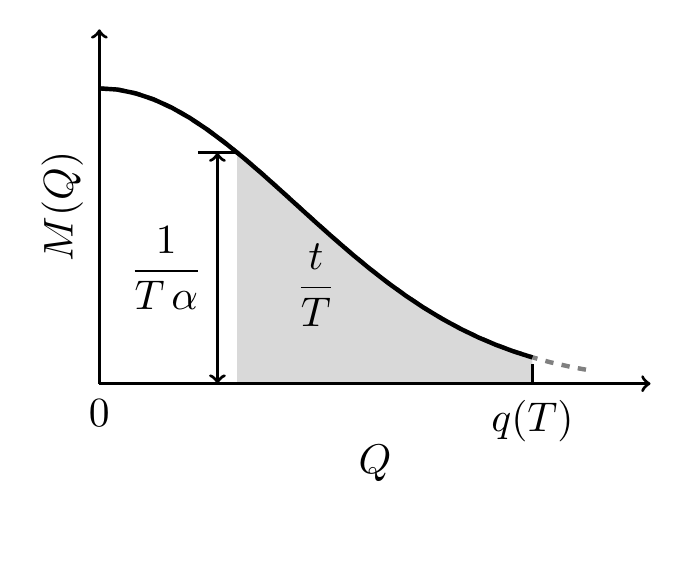
\begin{tikzpicture}[very thick, scale=2.5, every node/.style={scale=1.5}]
    % distribution
    \draw[domain=0:2.5, variable=\x, dashed, gray, ultra thick]
      plot({\x}, {1.5*exp(-0.5*\x*\x)});

    % shade
    \fill [gray!30!white, domain=0.7:2.2, variable=\x]
      (0.7, 0) --
      plot ({\x}, {1.5*exp(-0.5*\x*\x)})
      -- (2.2, 0) -- cycle;

    % thick curve
    \draw[domain=0:2.2, variable=\x, ultra thick]
      plot({\x}, {1.5*exp(-0.5*\x*\x)});

    % label for the shaded area
    \node[] at (1.1, 0.5) {$\dfrac{t}{T}$};

    \draw[<->] (0.6, 0)  --
               node[left, inner sep=1mm]
               {$\dfrac{1}{T \, \alpha}$}
               (0.6, 1.174);
    % label for the ordinate
    %\node[fill=white] at (0.4, 0.7) {$\dfrac{1}{Ta}$};

    \draw[] (0.5, 1.174) -- (0.7, 1.1740);
    \draw[->] (0, 0) -- node[below, inner sep=5mm] {$Q$} (2.8, 0);
    \draw[->] (0, 0) -- node[above, rotate=90] {$M(Q)$} (0, 1.8);

    % xtics
    \draw[] (0.0, 0.1) -- (0.0, 0.0) node[below] {$0$};
    \draw[] (2.2, 0.1) -- (2.2, 0.0) node[below] {$q(T)$};
  \end{tikzpicture}
  %\makebox[\linewidth][c]{
  %  \includegraphics[angle=0, width=0.9\linewidth]{fig/massq.pdf}
  %}
  \caption{
    \label{fig:massq}
    Geometric characterization of the optimal schedule,
    $\alpha(t)$,
    via the normalized mass distribution, $m(Q)$.
    %
    \note{
      The figure was produced by \texttt{tikz}.
      % Gnuplot version by doc/fig/massq.gp
    }%
  }
\end{center}
\end{figure}


Then, from Eq. \eqref{eq:q_opt},
we find that for $Q = q(T) - q(t)$,
%
\begin{align}
  m(Q)
  &=
  \frac{ 1 }
       { T \, \alpha(t) }
  ,
\label{eq:mQ_invTa}
  \\
  \int_Q^{ q(T) }
    m(Q') \, dQ'
  &=
  \frac t T
  ,
\label{eq:intmQ_tT}
\end{align}
%
which means that each point
$\bigl(t, \alpha(t)\bigr)$
on the schedule can be mapped
to a point
$\bigl(Q, m(Q)\bigr)$
on the mass distribution,
such that the ordinate of the latter curve
gives $1/(T\alpha)$,
and the area under the curve in the domain $[Q, q(T)]$
is equal to $t/T$,
as shown in Fig. \ref{fig:massq},

This mapping allows us to classify all optimal schedules
as follows.
%
We collect in each class optimal schedules
computed from simulations with the same function $M(Q)$
and cutoff value $q(T)$.
%
The former is determined by the values of
$\lambda_k$'s and $\Gamma_k$'s,
whereas the latter affects the distribution $m(Q)$
via the normalization constant $C$.


In each class, the updating magnitudes of two schedules
of lengths $T_1$ and $T_2$
at corresponding times $t_1/T_1 = t_2/T_2$
are related by $T_1 \, \alpha_1 = T_2 \, \alpha_2$.
%
Further, by Eqs.
\eqref{eq:error_asym_Lagrangian}
and
\eqref{eq:Lagrangian_const},
we have
%
\begin{equation}
  E_A
  =
  \frac { C^2 } { T }
  =
  \frac 1 T
  \left(
    \int_0^{ q(T) } M(Q) \, dQ
  \right)^2
  ,
\label{eq:error_asym2}
\end{equation}
%
which means the asymptotic error
is inversely proportional to the simulation length
for the same-class schedules,
i.e., we have the scaling relation
$T_1 \, E_{A1} = T_2 \, E_{A2}$.


%The optimal schedule has the following scaling property.
%%
%For two simulations of lengths $T_1$ and $T_2$,
%if $q(T_1) = q(T_2)$
%and they share the same $\lambda_k$'s and $\Gamma_k$'s,
%the updating magnitudes at the corresponding times,
%$t_1/T_1 = t_2/T_2$,
%can be related as $T_1 \, \alpha_1 = T_2 \, \alpha_2$.
%%
%In other words,
%if $\alpha(t_1)$ is
%an optimal schedule of the simulation of length $T_1$,
%then
%$\frac{T_1}{T_2} \alpha\left( \frac{ T_1 } { T_2 } t_2 \right)$
%is an optimal schedule of the simulation of length $T_2$.
%%
%The asymptotic errors are related by
%$T_1 \, E_{A1} = T_2 \, E_{A2}$.



\subsubsection{\label{sec:optinitalpha}
  Optimal initial updating magnitude
}


Let us now consider simulations in which
the system is initially equilibrated at the same
constant updating magnitude $\alpha_0$.
%
For these simulations,
we can adjust $q(T)$
to minimize the total error.
%
From Eqs. \eqref{eq:error_res1}
and \eqref{eq:error_asym2},
we find that
the $q(T)$ that minimizes
the total error satisfies
\begin{equation}
  m\bigl( q(T) \bigr)
  =
  \frac{1} { T \, (\alpha_0 / 2) }
  .
\label{eq:opt_qT}
\end{equation}
%
\note{Let $Q_c \equiv q(T)$,
$$
\begin{aligned}
  \frac{
    \partial E_R
  }
  {
    \partial q(T)
  }
  &=
  -\alpha_0 \, M^2(Q_c)
  ,
  \\
  \frac{
    \partial E_A
  }
  {
    \partial q(T)
  }
  &=
  \frac 2 T \,
  M(Q_c) \,
  \int_0^{ Q_c } M(Q) \, dQ
  .
\end{aligned}
$$
Then solve $\partial (E_R + E_A) / \partial q(T) = 0$.
}%
By Eqs. \eqref{eq:mQ_invTa} and \eqref{eq:intmQ_tT},
we can rewrite the condition as
\begin{equation}
  \alpha( t = 0 )
  =
  \frac{ \alpha_0 }
       { 2 }
  ,
\label{eq:half_alpha0}
\end{equation}
%
i.e., the optimal initial updating magnitude
is always half of the equilibration value.
%
This factor $1/2$
happens to coincide with the
reduction factor of updating magnitude
at stage transitions
in the original WL algorithm\cite{
wang2001, wang2001pre}.


Besides,
for simulations with the same $\alpha_0$,
Eq. \eqref{eq:opt_qT} shows that
the optimal $q(T)$ increases with
the simulation length $T$.
%
If $M(Q)$ decays rapidly,
the distribution $m(Q)$ does not critically
depend on the cutoff $q(T)$,
as long as $q(T)$ is sufficiently large.
%
So the optimal schedules of these simulations
approximately satisfy the scaling relations
described in Sec. \ref{sec:mass_distr}.
%
If, however, $M(Q)$ has a long tail
because of some near-zero $\lambda_k$'s,
increasing the simulation length $T$
generally alters the shape of the optimal schedule.




\subsection{\label{sec:band-matrix}
Homogeneous updating schemes}



Many commonly-used updating schemes
can be characterized by a rigid window
centered on the current bin.
%
We call these schemes homogeneous,
or translationally invariant.
%
An example is the Gaussian updating scheme
used in metadynamics.

By the translational invariance,
homogeneous updating schemes
satisfy detailed balance,
Eq. \eqref{eq:w_detailedbalance},
for the flat distribution, $\rho_i = 1/n$,
i.e., the updating matrix, $\mathbf w$,
is symmetric.
%
Besides, the updating matrices
share the same set of eigenvectors,
and thus are completely determined
by the eigenvalues.
%
Further, the multiplication of $\mathbf w$
can be reduced to a convolution with the window,
or the updating kernel.
%
Thus,
there is a one-to-one correspondence between
the eigenvalues of $\mathbf w$
and the updating kernel.



\subsubsection{\label{sec:bandkernel}
Updating kernel and eigenvalues}



%While translationally-invariant
%updating schemes
%naturally suit periodic variables\cite{
%dama2014},
%they can also be extended to non-periodic variables
%by imposing the reflective boundary condition\cite{
%bussi2006}.
%%
%For simplicity, we shall assume that the target
%distribution is flat, or $p_i = 1/n$, below.



It is natural to first introduce homogeneous updating schemes
for a periodic variable\cite{dama2014}.
%
The updating matrix, $\mathbf w$,
assume the following form
%
\begin{equation}
  w_{ij}
  =
  \mu_{i-j}
  +
  \mu_{i-j+n}
  +
  \mu_{i-j-n}
  ,
\notag
%\label{eq:w_band_pbc}
\end{equation}
%
where
$\mu_{-b}, \dots, \mu_b$ ($b \le n/2$)
are a set of numbers satisfying
%
\begin{equation}
  \mu_{-b} + \cdots + \mu_b = 1
  ,
\label{eq:mu_normalization}
\end{equation}
%
and $\mu_l = 0$ for $|l| > b$.
%
Particularly,
we shall only consider symmetric kernels
that satisfy
%
\begin{equation}
  \mu_i = \mu_{-i}
  .
\label{eq:mu_symm}
\end{equation}
%
If $b = n/2$, then $\mu_{-b}$ is removed
from the sum in Eq. \eqref{eq:mu_normalization}
to avoid double counting.
%
These numbers constitutes an \emph{updating kernel}.


The above matrix, $\mathbf w$,
being symmetric to the indices $i$ and $j$,
satisfies Eqs. \eqref{eq:w_sumj}-\eqref{eq:w_balance},
for the flat distribution.
%
To find the eigenvectors,
we define, for a periodic variable, $\phi_i$,
the out-of-boundary values by
%
\begin{equation}
  \phi_i = \phi_{i \pm n},
\label{eq:phi_pbc}
\end{equation}
%
such that $i \pm n$ lies in between $1$ and $n$.
%
Then
%
\begin{equation}
  \sum_{ j = 1 }^n
    w_{ij} \, \phi_j
  =
  \sum_{ j = 1 - n }^{ 2 \, n }
    \mu_{i - j} \, \phi_j
  =
  \sum_{ l = -b }^{ b }
    \mu_l \, \phi_{ i - l}
  .
\label{eq:wmul_to_convol}
\end{equation}
%
\note{The derivation of the first step of
  Eq. \eqref{eq:wmul_to_convol}:
$$
\begin{aligned}
  \sum_{j = 1}^n
    w_{ij} \, \phi_j
  &=
  \sum_{j = 1}^n
    \mu_{i - j} \, \phi_j
  +
  \sum_{j = 1}^n
    \mu_{i - j - n} \, \phi_j
  +
  \sum_{j = 1}^n
    \mu_{i - j + n} \, \phi_j
  \\
  &=
  \sum_{j = 1}^n
    \mu_{i - j} \, \phi_j
  +
  \sum_{j = 1+n}^{2 \, n}
    \mu_{i - l} \, \phi_l
  +
  \sum_{j = 1-n}^0
    \mu_{i - j + n} \, \phi_j
  \\
  &=
  \sum_{j = 1-n}^{2 \, n}
    \mu_{i - j} \, \phi_j
  .
\end{aligned}
$$
The second step of Eq. \eqref{eq:wmul_to_convol}
follows from the constraint $\mu_l = 0$ for $|l| > b$.

Similarly,
for the left eigenvector, we have
$$
  \sum_{ i = 1 }^n
    \phi_i \, w_{ij}
  =
  \sum_{ l = -b }^b
    \phi_{j - l} \, \mu_{-l}
  .
$$
But due to the symmetry Eq. \eqref{eq:mu_symm},
it is identical to \eqref{eq:wmul_to_convol}.
}

Thus,
we may construct a set of orthonormal eigenvectors,
$\pmb\phi^{(1)}, \dots, \pmb\phi^{(n)}$,
compatible with Eq. \eqref{eq:phi_pbc},
\begin{equation}
  \phi^{(k)}_j
  =
  \phi_{kj}
  =
  \frac 1 n
  \exp
  \left[
    \ii
    \frac{ (k - 1) \, j \, 2 \, \pi }
         {            n             }
  \right]
  ,
  \notag
\end{equation}
%
where $\ii^2 = -1$, and
the eigenvalues are
%
\begin{equation}
  \lambda_k
  =
  \mu_0
  +
  2 \,
  \sum_{ l = 1 }^b
  \mu_l
  \cos
  \frac{ (k - 1) \, l \, 2 \, \pi }
       {            n             }
  .
  \label{eq:wband_eigenvalue_pbc}
\end{equation}
%
\note{Consider the unnormalized version
  $$
  \Phi^{(k)}_j =
  \exp\left[
    \frac{ ( k - 1 ) \, j \, 2 \, \pi }
         {              n             }
    \ii
  \right]
  ,
  $$
  we have
  $$
  \begin{aligned}
  \sum_{j = 1}^n
    w_{ij} \, \Phi^{(k)}_j
  &=
  \sum_{l = -b}^b
    \mu_l \, \Phi^{(k)}_{i - l}
  \\
  &=
  \mu_0 \, \Phi^{(k)}_i
  +
  \sum_{l = 1}^b
    \mu_l \,
    \left[ \Phi^{(k)}_{i - l} + \Phi^{(k)}_{i + l} \right]
  \\
  &=
  \Phi^{(k)}_i \,
  \left[
    \mu_0
    +
    2 \sum_{l = 1}^b
      \mu_l \, \cos
      \frac{ (k - 1) \, l \, 2 \, \pi }
           {            n             }
  \right]
  .
  \end{aligned}
  $$
  The term in the square brackets is the eigenvalue given by
  Eq. \eqref{eq:wband_eigenvalue_pbc}.
}
%
Note, however, the two-fold degeneracy as
$\lambda_{n - k + 2} = \lambda_k$.



To adapt the above formulae to a non-periodic variable,
we use the reflective boundary condition\cite{bussi2006},
and change the form of the updating matrix to
%
%
\begin{equation}
  w_{ij}
  =
  \mu_{ i - j }
  +
  \mu_{ i + j - 1 }
  +
  \mu_{ i + j - 2 n - 1 },
  \label{eq:w_band_refl}
\end{equation}
%
Again the updating kernel should satisfy
Eqs. \eqref{eq:mu_normalization}
and \eqref{eq:mu_symm},
but
the cutoff $b$ only need to be less than $n$.
%
The last two terms
on the right-hand side of Eq. \eqref{eq:w_band_refl} are added
to avoid unintended distortion\cite{dickson2011, mcgovern2013}
to the equilibrium distribution\cite{bussi2006},
such that Eqs. \eqref{eq:w_sumj}-\eqref{eq:w_balance}
are satisfied.

Parallel to Eq. \eqref{eq:phi_pbc},
we define the out-of-boundary values
of $\phi_i$ as
%
\begin{equation}
  \phi_i
  =
  \begin{dcases}
    \phi_{ 1 - i }           & \mathrm{for \;} i \le 0, \\
    \phi_{ 2 \, n + 1 - i }  & \mathrm{for \;} i > n,
  \end{dcases}
\label{eq:phi_refl}
\end{equation}
%
such that Eq. \eqref{eq:wmul_to_convol}
still holds.
%
\note{The derivation of Eq. \eqref{eq:wmul_to_convol}
  in this case is similar,
  $$
  \begin{aligned}
    \sum_{j = 1}^n w_{ij} \, \phi_j
    &=
    \sum_{j = 1}^n
      \mu_{i - j} \, \phi_j
    +
    \sum_{j = 1}^n
      \mu_{i + j - 1} \, \phi_j
    +
    \sum_{j = 1}^n
      \mu_{i + j - 2 \, n - 1} \, \phi_j
    \\
    &=
    \sum_{j = 1}^n
      \mu_{i - j} \, \phi_j
    +
    \sum_{l = 1 - n}^0
      \mu_{i - l} \, \phi_l
    +
    \sum_{l = n + 1}^{ 2 \, n }
      \mu_{i - l} \, \phi_l
    \\
    &=
    \sum_{j = 1 - n}^{ 2 \, n}
      \mu_{i - j} \, \phi_j.
  \end{aligned}
  $$
}%
Thus, we also have $n$ orthonormal eigenvectors,
$\pmb\phi^{(1)}, \dots, \pmb\phi^{(n)}$,
compatible with Eq. \eqref{eq:phi_refl},
%
\begin{equation}
  \phi^{(k)}_i
  =
  \phi_{k i}
  =
  \frac{ \sqrt{ 2 - \delta_{k, 1} } }
       {             n              }
  \cos \frac{ ( k - 1) \, \left( i - \frac 1 2 \right) \, \pi}
            {                    n                           }
  ,
\notag
%\label{eq:wband_eigenvector_refl}
\end{equation}
%
with eigenvalues
%
\begin{align}
  \lambda_k
  &=
  \mu_0
  +
  2
  \sum_{l = 1}^b
    \mu_l
    \cos \frac{(k - 1)  \, l \pi}{n}
  .
\label{eq:wband_eigenvalue_refl}
\end{align}
%
\note{Derivation.
  First consider the unnormalized eigenvectors,
  $$
  \Phi^{(k)}_i
  =
  \cos \frac{ \left( i - \frac 1 2 \right) (k - 1) \, \pi}{n},
  $$
  which satisfies Eq. \eqref{eq:phi_refl}.
  %
  So, by Eq. \eqref{eq:wmul_to_convol},
  $$
  \begin{aligned}
  \sum_{i = 1}^n
    \Phi^{(k)}_i \, w_{ij}
  &=
  \sum_{l = -b}^b
    \Phi^{(k)}_{j - l} \, \mu_l
  \\
  &=
    \Phi^{(k)}_j \, \mu_0
  + \sum_{l=0}^{b}
    \mu_l \,
    \left[
      \Phi^{(k)}_{j-l}
      +
      \Phi^{(k)}_{j+l}
    \right]
  \\
  &= \Phi^{(k)}_j \, \lambda_k,
  \end{aligned}
  $$
  with $\lambda_k$ given by Eq. \eqref{eq:wband_eigenvalue_refl}.
}%


Note that Eq. \eqref{eq:wband_eigenvalue_refl}
differs from Eq. \eqref{eq:wband_eigenvalue_pbc}
by a factor of $2$
in the argument of the cosine function.
%
We may unify the two as
%
\begin{equation}
  \lambda_k
  =
  \mu_0
  +
  2
  \sum_{ l = 1 }^b
    \mu_l \,
    \cos \frac{ (k - 1) \, l \, g \, \pi }
              {            n             }
  ,
  \label{eq:wband_eigenvalue}
\end{equation}
%
where the degeneracy $g$ is $2$
for the periodic case,
or $1$ otherwise.
%
In both cases,
the eigenvalues, $\lambda_k$'s,
is the cosine transform of
the updating kernel.
%
For the updating scheme to be stable,
the cosine transform of the kernel
must be nonnegative.
%
If this is not so,
we can modify the kernel
using the technique described
in Appendix \ref{sec:stabilize_wband}.

We discuss two special cases below.



\subsubsection{\label{sec:nnscheme}
Triple-bin updating scheme}



If $\mu_2 = \dots = \mu_b = 0$,
the matrix $\mathbf w$ is tridiagonal,
%%
%\begin{equation}
%\arraycolsep=3.6pt\def\arraystretch{1.4}
%\mathbf w
%=
%\left(
%  \begin{array}{cccccccc}
%    1 - \mu_1   & \mu_1 & 0 & \dots & 0 \\
%    \mu_1 & 1 - 2 \, \mu_1  & \mu_1 & \dots & 0 \\
%    \vdots & &  & & \vdots \\
%    0 & \dots & \mu_1 & 1 - 2 \, \mu_1  & \mu_1 \\
%    0 & \dots & 0 & \mu_1 & 1 - \mu_1
%  \end{array}
%\right).
%\label{eq:wnn}
%\end{equation}
%%
%We have
and the eigenvalues are
\begin{equation}
  \lambda_k
  =
  1 -
  4 \, \mu_1 \sin^2
  \frac{ (k - 1) \, g \, \pi }
       {       2 \, n        }
  .
\notag
%\label{eq:wnn_eigenvalue}
\end{equation}
%
So this updating scheme is stable if
$\min \lambda_k = \lambda_n \ge 0$,
or
\begin{equation}
  \mu_1 \le
  \begin{dcases}
    \frac 1 4
    & \mathrm{periodic \; and \;} n \mathrm{ \; even,}
    \\
    \frac 1 4
    \sec^2
    \left( \frac{  \pi   }
                { 2 \, n }
    \right)
    & \mathrm{otherwise}.
  \end{dcases}
\notag
%\label{eq:nn_stable}
\end{equation}






\subsubsection{Gaussian updating scheme}



The Gaussian updating scheme is commonly
used in metadynamics simulations.
%
Below we shall show its stability
in the continuous limit.



For $n \gg 1$,
we define
$x = l \, g \, \Delta x$,
and
$\mu_l = \mu(x) \, \Delta x$,
where
$\Delta x = \pi/n$
is the bin size.
%
By assuming the largest $b \approx n/g$,
Eq. \eqref{eq:wband_eigenvalue}
can be approximated as an integral:
%
\begin{equation}
  \lambda_k
  =
  2 \int_0^\pi
    \mu(x) \, \cos \bigl[ (k-1) \, x \bigr] \, dx,
\notag
%\label{eq:lambda_int}
\end{equation}
%
with the normalization
%
$
  1 = 2 \int_0^\pi \mu(x) \, dx.
$


For the Gaussian updating kernel,
if the width $\sigma$ satisifies
with $\Delta x \ll \sigma \ll 1$,
we can extend
the upper limit of the integrals
to infinity, and
%
\begin{equation}
  \mu(x)
  =
  \frac{            1            }
       { \sqrt{ 2 \pi \sigma^2 } }
  %
  \exp\left(
        -\frac{       x^2     }
              { 2 \, \sigma^2 }
      \right)
  .
\notag
\end{equation}
%
%
If follows that all eigenvalues are positive:
%
\begin{align}
  \lambda_k
  &=
  \exp\left[
        -\frac{ (k - 1)^2 \, \sigma^2 }
              {           2           }
      \right]
  %\notag
  %\\
  %&=
  %\exp\left[
  %      -\frac{ \pi^2 }{ 2 }
  %      \left(
  %        \frac{ k - 1 }
  %             {   n   }
  %      \right)^2
  %      \left(
  %        \frac{  \sigma }
  %             { \Delta x }
  %      \right)^2
  %    \right]
  .
\notag
%\label{eq:lambda_Gaussian}
\end{align}



%However,
%as $\sigma/\Delta x \gg 1$,
%the smallest eigenvalue
%%
%$$
%\lambda_n
%\approx
%\exp\left(
%      -\frac{ n^2 \, \sigma^2 }
%            {        2        }
%    \right)
%=
%\exp\left[
%      -\frac{ \pi^2 }{ 2 }
%      \left(
%        \frac{  \sigma }
%             { \Delta x }
%      \right)^2
%    \right]
%.
%$$
%%
%is exponentially small.
%%
%This means that
%the optimal value of $\lambda$
%given by Eq. \eqref{eq:optimal_lambda_approx}
%would be too small in practice,
%for it requires $\lambda < 2 \, \lambda_n$.
%%
%In other words,
%with a reasonable $\lambda$,
%the error of the last few fluctuation modes
%will always decay suboptimally,
%accordingly to Eq. \eqref{eq:error_asym_invt}.
%%
%However, since these modes
%represent short wavelength fluctuations,
%and these modes may be in
%the system under consideration.
%%
%Thus,
%we can truncate the sum of the error function
%in Eq. \eqref{eq:error_asym_invt}
%at some $k_{\max}$,
%which corresponds to a minimal length scale
%$l_{\min} = \Delta x \, (n /k_{\max}) = \pi/k_{\max}$
%greater than $\sigma$.
%%
%Then,
%$$
%\lambda_{ k_{\max} }
%\approx
%\exp\left(
%      -\frac{ k_{\max}^2 \, \sigma^2 }
%            {           2            }
%    \right)
%=
%\exp\left(
%      -\frac{  \pi^2 \, \sigma^2    }
%            {    2 \, l_{\min}^2  }
%    \right).
%$$



\subsubsection{\label{sec:invert_wband}
Inversion}



Since the eigenvalues are related to the updating kernel
by a cosine transform,
Eq. \eqref{eq:wband_eigenvalue},
the relation can be readily inverted.
%
In the periodic case,
we have
%the inversion formula is
%
\begin{equation}
  \mu_l
  =
  \frac 1 n
  \sum_{ k = 1 }^n
  \lambda_k
  \cos \frac{ (k - 1) \, l \, 2 \, \pi }
            {            n             }
  .
\label{eq:mu_from_lambda_pbc}
\end{equation}


In the non-periodic case,
the formula is
%
\begin{align}
  \mu_l
  =
  \frac 1 { 2 \, n }
  \sum_{ k = 1 }^{ 2 \, n }
    \lambda_{ k } \,
    \cos \frac{ (k - 1) \, l \, \pi }
              {            n        }
  ,
\label{eq:mu_from_lambda_refl}
\end{align}
%
where
we have defined
$\lambda_k \equiv \lambda_{2 \, n + 2 - k}$
for $k = n + 2, \dots, 2 \, n$,
as well as
%
\begin{align}
  \lambda_{ n + 1 }
  =
  (-1)^{ n - 1 }
  \lambda_1
  +
  2 \, \sum_{ k = 2 }^{ n }
      (-1)^{n - k} \, \lambda_k
  ,
\label{eq:lambdan}
\end{align}
to satisfy the constraint $\mu_n = 0$.
%
\note{Eq. \eqref{eq:lambdan}
  ensures that the $\mu_n$
  computed from Eq. \eqref{eq:mu_from_lambda_refl}
  vanishes.

  %The inversion formula is derived from the cosine transform.
  %
  If we define $\mu_n = 0$ and
  %
  $
    \mu_{ 2 n - l } = \mu_l,
  $
  for
  $l = 1, \dots, n - 1$,
  %
  then Eq. \eqref{eq:wband_eigenvalue_refl} can be rewritten as
  %
  \begin{align}
    \lambda_{k+1}
    =
    \sum_{ l = 0 }^{ 2 \, n - 1 }
    \mu_l \, \cos \frac{ k \, l \, \pi } { n }.
  \notag
  %\label{eq:lambda_cosine_sum}
  \end{align}
  %
  This formula for $\lambda_{k+1}$
  can be readily extended to $k = 2 \, n - 1$,
  and we have
  %
  $
    \lambda_{ 2 \, n + 2 - k } = \lambda_k
    .
  $
  %
  Thus,
  %
  $$
  \begin{aligned}
    \sum_{ k = 0 }^{ 2 \, n - 1 }
      \lambda_{ k + 1 } \,
      \cos \frac{ k \, p \, \pi }
                {      n        }
    &=
    \sum_{ k = 0 }^{ 2 \, n - 1 }
      \sum_{ l = 0 }^{ 2 \, n - 1 }
        \mu_l \,
        \cos \frac{ k \, l \, \pi }
                  {      n        }
        \cos \frac{ k \, p \, \pi }
                  {      n        }
    \\
    &=
    \sum_{ l = 0 }^{ 2 \, n - 1 }
      \frac{ \mu_l } { 2 }
      \sum_{ k = 0 }^{ 2 \, n - 1 }
        \cos \frac{ k \, (p + l) \, \pi }
                  {      n        }
                  +
        \cos \frac{ k \, (p - l) \, \pi }
                  {      n        }
    \\
    &=
    \sum_{ l = 0 }^{ 2 \, n - 1 }
      \mu_l \, n \left(
        \delta_{ p + l - 2 \, n, 0 }
        +
        \delta_{ p - l, 0 }
      \right)
    \\
    &=
    n \, \left( \mu_p + \mu_{ 2 \, n - p} \right)
    =
    2 \, n \, \mu_p.
  \end{aligned}
  $$
  This entails Eq. \eqref{eq:mu_from_lambda_refl}.
  %
  The value of $\lambda_{n + 1}$
  can be deduced from
  imposing $\mu_n = 0$
  and solving Eq. \eqref{eq:mu_from_lambda_refl}
  for $l = n$,
  yielding Eq. \eqref{eq:lambdan}.
}



\subsection{\label{sec:cmpschemes}
Comparison of updating schemes}


Now that we can compute the optimal schedule
for a given updating scheme,
we shall turn to the problem of choosing
optimal updating schemes below.


\subsubsection{\label{sec:optWL}
Asymptotic optimality of the single-bin scheme}



We shall first show
that the single-bin scheme is asymptotically optimal.
%
Consider a class of $\mathbf w$ matrices
sharing the same set of eigenvectors,
hence the same $\Gamma_k$'s,
but with different positive eigenvalues,
$\lambda_k$'s.
%
Using the Cauchy-Schwarz inequality, we have,
for any set of nonnegative numbers, $c_k$'s,
%
\begin{align}
&
\left(
  \int_0^T dt
    \sum_{k = 2}^n
      \Gamma_k \, \dot u_k^2\bigl( q(t) \bigr)
\right)
%
\left(
  \int_0^T dt
    \sum_{k = 2}^n
      \Gamma_k \, c_k^2
\right)
%
\notag
\\
&
\qquad \qquad
\ge
\left(
  \int_0^T dt
    \sum_{k = 2}^n
      \Gamma_k \, c_k \, \dot u_k \, \bigl( q(t) \bigr)
\right)^2
\notag
\\
&
\qquad \qquad
=
\left(
  \sum_{k = 2}^n \Gamma_k \, c_k
    \left[
      1 - e^{ -\lambda_k \, q(T) }
    \right]
\right)^2.
\label{eq:CSineq}
\end{align}
%
\note{This inequality follows from the non-negativity of
the following quadratic polynomial of $Y$,
$$
\int_0^T
  dt \sum_{k = 2}^n \Gamma_k \,
    \left( \dot u_k \, Y - c_k \right)^2
  \equiv
  A \, Y^2 + B \, Y + C
  ,
$$
which implies a non-positive discriminant,
$B^2 - 4 \, A \, C$.
}%
%
Note that the last expression of \eqref{eq:CSineq}
depends on the curve, $q(t)$ ($0 < t < T$),
only through the endpoint value, $q(T)$,
which is fixed in the variational process.
%
Thus, the inequality sets a lower bound
for the asymptotic error $\Err$
given in Eq. \eqref{eq:error_asym1}.
%
The equality is achieved
if $\dot u_k\left( q(t) \right) = c_k$
for all $k = 2, \dots, n$ at any $t$,
up to a multiplicative factor.
%
Solving these equations yields
%
\begin{equation}
  \alpha(t) = \frac{              1             }
                   { \lambda_k \, (t + t_{k0} ) },
\label{eq:alpha_invtk}
\end{equation}
with
\begin{equation}
  t_{k0} = \frac{             T            }
                { e^{ \lambda_k q(T) } - 1 }.
\label{eq:tk0}
\end{equation}
%
Such a solution is possible only if
%
\begin{equation}
  \lambda_2 = \dots = \lambda_n.
  \notag
\end{equation}
%
Then, by Eq. \eqref{eq:tk0},
all $t_{k0}$'s also share the same value,
$t_0$,
such that
$u_k = (t + t_0) / (T + t_0)$,
and
$c_k = 1/(T + t_0)$
for $k \ge 2$.
%
The asymptotic error is then
\begin{align}
  E_A
  =
  \frac{       T     }
       { (T + t_0)^2 }
  \sum_{ k = 2 }^n
    \Gamma_k
  .
\label{eq:error_singlebin}
\end{align}
%
If we further assume $\lambda_2 = 1$,
%the optimal schedule given by
Eq. \eqref{eq:alpha_invtk}
recovers Eq. \eqref{eq:alpha_invt1}.
%
\note{Derivation.
  Integrating $\dot u_k = c_k$ yields
  \begin{equation}
    u_k(t) = c_k \left(t + t_{k0} \right).
  \tag{UK}
  \label{neq:ui_solution}
  \end{equation}
  Given that $u_k(T) = 1$ and $u_k(0) = e^{-\lambda_k \, q(T)}$,
  we have
  $$
  c_k = \frac{ 1 }{ T + t_{k0} },
  \quad
  \mathrm{and\;}
  \frac{ t_{k0} } { T + t_{k0} }
  =
  e^{ -\lambda_k \, q(T) }.
  $$
  Taking the logarithm of Eq. \eqref{neq:ui_solution} yields
  $$
  -\lambda_k \, q(T) + \lambda_k \, q(t)
  = \ln c_k + \ln \left( t + t_{k0} \right).
  $$
  Differentiating this with respect to $t$ yields
  Eq. \eqref{eq:alpha_invtk}.
}

Since the first eigenmode corresponds to
a uniform shift of all $v_k$'s,
we can freely set $\lambda_1$ to $\lambda_2$
without changing the nature of the updating scheme.
%
Now an updating matrix
with identical eigenvalues
is a multiple of the identity matrix.
%
Thus,
the single-bin scheme is most efficient
in asymptotic convergence.
%if no eigenvalue $\lambda_k$ is zero.



\subsubsection{\label{sec:optscheme}
Bandpass updating schemes}


We can generalize
the single-bin scheme to a class of
perfect (brick-wall) \emph{bandpass} updating schemes
to allow zero eigenvalues.
%
For example,
%if we can assume
by assuming
that the PMF is sufficiently smooth
such that the eigenmodes can be limited to $k \le K$,
%
we can construct an updating scheme with
$$
\lambda_1 = \cdots = \lambda_K = 1,
\mathrm{\; and \;}
\lambda_{K+1} = \cdots = \lambda_n = 0.
$$
%
Then,
we can change the upper limit of the sum in
Eq. \eqref{eq:error_singlebin} to $K$.
%
%Then,
%Eq. \eqref{eq:error_singlebin} is changed to
%%
%\begin{equation}
%  E_A
%  =
%  \frac {       T     }
%        { (T + t_0)^2 }
%  \sum_{ k = 2 }^K
%    \Gamma_k.
%%\notag
%\label{eq:error_asym_sinc}
%\end{equation}
%
The optimal schedule of these schemes
remains to be the inverse-time one
given by Eq. \eqref{eq:alpha_invt1}.
%
Below, we construct these schemes for
the homogeneous case.

For a periodic variable, we demand
%
$$
\begin{aligned}
&
\lambda_1 = \cdots = \lambda_{K+1}
= \lambda_{n-K+1} = \cdots = \lambda_n = 1,
\\
&
\lambda_{K+2} = \cdots = \lambda_{n-K} = 0,
\end{aligned}
$$
for $K \ge 1$.
%
Then by using
Eq. \eqref{eq:mu_from_lambda_pbc},
we get
\begin{equation}
  \mu_l
  =
  \frac{
    \sin
    \dfrac{ (2 K + 1) \, l \, \pi }
         {              n        }
  }
  {
    n \, \sin \dfrac{ l \, \pi } { n }
  }
  .
\notag
%\label{eq:mu_sinc_pbc}
\end{equation}
\note{Derivation.
$$
\begin{aligned}
\mu_l
&=
\frac 1 n \sum_{k = 0}^{n-1} \lambda_{k+1} \cos \frac{ k \, l \, 2 \, \pi } { n }
\\
&=
\frac{1}{n}
\left(
  1 +
  \sum_{k=1}^K
  \cos \frac { k \, l \, 2 \, \pi } { n }
  +
  \sum_{k=n-K}^{n-1}
  \cos \frac { k \, l \, 2 \, \pi } { n }
\right)
\\
&=
\frac 1 n
\sum_{k=-K}^K
\cos \frac { k \, l \, 2 \, \pi } { n }
=
  \frac{
    \sin
    \dfrac{ (2 K + 1) \, l \, \pi }
         {              n        }
  }
  {
    n \, \sin \dfrac{ l \, \pi } { n }
  }
.
\end{aligned}
$$
}

For a non-periodic variable, we demand
$$
\lambda_1 = \cdots = \lambda_{K+1} = 1,
\qquad
\lambda_{K+2} = \cdots = \lambda_n = 0.
$$
Then Eq. \eqref{eq:lambdan} gives
$\lambda_{n+1} = (-1)^{n+K-1}$,
and from Eq. \eqref{eq:mu_from_lambda_refl},
we have
\begin{equation}
  \mu_l
  =
  \frac{1}{2 \, n}
  \left[
    (-1)^{n+K+l-1}
    +
    \frac{
      \sin
      \dfrac{ (2 K + 1) \, l \, \pi }
           {         2 \, n        }
    }
    {
      \sin \dfrac{ l \, \pi } { 2 \, n }
    }
  \right]
  .
\label{eq:mu_sinc_refl}
\end{equation}
\note{Derivation.
$$
\begin{aligned}
  \lambda_{n+1}
  &=
  (-1)^{n-1}
  \left[
    \lambda_1
    - 2 \, \lambda_2
    + 2 \, \lambda_3 - \cdots
    + (-1)^{K} 2 \, \lambda_{K+1})
  \right]
  \\
  &=
  \begin{dcases}
    (-1)^{n-1} & K \mathrm{\; even,} \\
    (-1)^n     & K \mathrm{\; odd.}
  \end{dcases}
\end{aligned}
$$
So
$$
\begin{aligned}
  \mu_l
  &=
  \frac{1}{2\,n}
  \left[
    1 +
    2 \sum_{k=2}^{K+1}
    \cos \frac { (k - 1) \, l \pi } { n }
    +
    (-1)^{n+K-1} (-1)^l
  \right]
  \\
  &=
  \frac{1}{2\,n}
  \left[
    (-1)^{n+K+l-1}
    +
    \sum_{k=-K}^{K}
    \cos \frac { k \, l \pi } { n }
  \right]
  .
\end{aligned}
$$
}%


\begin{figure}[h]
\begin{center}
  \makebox[\linewidth][c]{
    \includegraphics[angle=0, width=0.95\linewidth]{fig/sinc.pdf}
  }
  \caption{
    \label{fig:sinc}
    Updating kernels of the bandpass updating schemes
    compared to a Gaussian with a similar width.
    %
    The lines are a guide to the eyes.
    Inset. Updating matrix in the non-periodic case.
    %
    \note{This figure was produced by \texttt{doc/fig/sinc.gp}.
      The data were computed by the program \texttt{prog/predict},
      see particularly the function \texttt{intq\_save()}
      in \texttt{prog/intq.h} for panel (a),
      and the functions \texttt{savewin()}
      and \texttt{savewinmat()}
      in \texttt{prog/invt.h} for panel (b),
      The data were saved under the directory \texttt{data/sinc}.
      See the \texttt{make} object \texttt{sincsingle}
      in the \texttt{Makefile} there.
    }%
  }
\end{center}
\end{figure}


In Fig. \ref{fig:sinc},
we give examples of the updating kernels
of the bandpass updating schemes,
compared to a Gaussian
with a similar width, $\sigma$,
%
\begin{equation}
  \sigma
  \approx
  \frac
  {
    n
  }
  {
    \sqrt{ 2 \, \pi } \, g \, K
  }
  .
\label{eq:sigma_equiv}
\end{equation}
%
%where $g = 2$ for the periodic case
%or $g = 1$ otherwise.
%
The kernel in the non-periodic case is a zigzag
because of the term $(-1)^{n+K+l-1}$
in Eq. \eqref{eq:mu_sinc_refl}.
%
However, as shown in the inset, % of Fig. \ref{fig:sinc}(b),
the ruggedness disappears
in the updating matrix by Eq. \eqref{eq:w_band_refl},
as the above oscillatory term for $l = i - j$
is canceled by the term for either $l = i + j - 1$
or $l = i + j - 2 \, n - 1$
with the opposite sign.



\subsubsection{\label{sec:finlencorr}
Finite-length correction}



In the above, we have focused on
the asymptotic error.
%
By including the residual error
and minimize the total,
we get the optimal $t_0$,
which is, according to Eq. \eqref{eq:half_alpha0},
%
%%Assuming the system is initially equilibrated
%%under a constant updating magnitude,
%%$\alpha_0$,
%Assuming Eq. \eqref{eq:error_res1} with
%$$
%q(T)
%=
%\int_0^T \frac{ dt } { t + t_0 }
%=
%\ln \frac{ T + t_0 } { t_0 }.
%$$
%%
%we have, from Eqs. \eqref{eq:error_split}
%and \eqref{eq:error_asym_sinc},
%%
%\begin{equation}
%  E
%  =
%  E_R + E_A
%  =
%  \frac { \frac 1 2 \alpha_0 \, t_0^2 + T }
%        {          ( T + t_0 )^2          }
%  \sum_{ k = 2 }^K \Gamma_k
%  .
%\notag
%%\label{eq:error_sinc0}
%\end{equation}
%%
%The minimum is reached at
%
\begin{equation}
  t_0
  =
  \frac{     2    }
       { \alpha_0 }
  ,
\label{eq:t0_sinc}
\end{equation}
%
and at this point
%
\begin{equation}
  E
  =
  \frac{   1     }
       { T + t_0 }
  \sum_{ k = 2 }^K
    \Gamma_k
  .
\label{eq:error_sinc}
\end{equation}
%
In Appendix \ref{sec:equilerr},
we show that the above error tends
to the error of the ideal equilibrium FDS simulation
in the asymptotic limit.





%
%For example, consider a system that is initially
%prepared under a fixed $\alpha_0$
%at the beginning of the schedule $\alpha(t)$.
%%
%Then for shorter times, $T \approx 0$,
%the error, dominated by the residual error
%given by Eq. \eqref{eq:error_res1},
%is clearly smaller if some eigenvalues
%are less than $1.0$ (the single-bin case).
%
%In practice, real simulations
%may have long achieved the desired precision
%before reaching the asymptotic regime,
%especially if the updating matrix
%has some $\lambda_k$'s close to $0$.




\section{\label{sec:results}
Numerical results}



We tested the above theory on a model system
described in Sec. \ref{sec:results_system}.
%
First, we verify the method of computing errors
%using an inverse-time schedule
in Sec. \ref{sec:results_invt}.
%
We then study the optimal schedule from
Eq. \eqref{eq:q_opt}
in Sec. \ref{sec:results_optschedule}.
%
Finally, we compare the Gaussian and
bandpass updating schemes %of different widths
in Sec. \ref{sec:results_cmpschemes}.



\subsection{\label{sec:results_system}
Test system and simulation protocol}



In our test system,
$i$ represents a one-dimensional
non-periodic variable,
and $n = 100$.
%
Both the target and intrinsic distributions
are assumed to be flat:
$p^*_i = p_i = 1/n$.
%
%We wish to see how
%the schedule, $\alpha(t)$,
%affects the fluctuating error
%of the bias potential
%at the end of the simulation.
%
Initially,
we set the bias potential to zero,
$V_i \equiv 0$,
and equilibrate the system for $10^7$ steps
under a constant updating magnitude,
$\alpha_0 = 10^{-4}$.
%
After this,
we reset the origin of the time, $t$,
and start the testing schedule
for $T = 10^8$ steps.
%
We repeat the above process $1000$ times
and average the results.
%specified by either
%Eq. \eqref{eq:q_opt}
%or
%Eq. \eqref{eq:alpha_invtlambda}.
Unless specified otherwise,
the above parameters were used.



For the Gaussian updating scheme,
the kernel was truncated at
$b = \min\{10 \, \sigma, n - 1\}$
and numerically stabilized
using the technique
in Appendix \ref{sec:stabilize_wband}.



%Since the error depends on
%the underlying sampling process,
We tested two sampling processes.
%a global one and a local one.
%
Both are based on
Metropolis MC algorithm\cite{
  metropolis1953, newman, frenkel,
  landau_binder}:
%
in each step, a new bin index $j$ is proposed
and then accepted with probability
%
$
A(i \to j) = \min\{ 1, \exp(V_i - V_j) \}.
$
However,
in the first or global sampling process,
we choose the destination $j$
uniformly out of the $n$ bins.
%
In the second or local sampling process,
$j$ is either $i - 1$ or $i + 1$
(adjusted by the boundary condition)
with equal probability $1/2$.
%
Asymptotically,
the above global and local sampling processes
emulate the perfect and one-step processes
discussed in Appendix \ref{sec:Gamma},
respectively,
and we shall use
Eqs. \eqref{eq:Gamma_perfect}
and \eqref{eq:Gamma_onestep}
for the respective $\Gamma_k$'s
in the theoretical predictions.
%



\subsection{\label{sec:results_invt}
Modified inverse-time schedule}


We tested the theory of computing errors
on the modified inverse-time schedule,
%
\begin{equation}
\alpha(t) = \frac{1}{\lambda \, (t + t_0) },
\label{eq:alpha_invtlambda}
\end{equation}
%
where $\lambda$ is a free parameter,
and $t_0$ is given by Eq. \eqref{eq:t0_sinc}.
%and $t_0 = 2/\alpha_0$.
%
The error of this schedule
can be computed analytically
(cf. Appendix \ref{sec:invt_schedule}),
and tested against simulation.



We performed adaptive FDS simulations
using the single-bin updating scheme
and the triple-bin updating scheme with $\mu_1 = 0.24$.
%
%For each value of $\lambda$,
%we ran $1000$ independent simulations
%of $10^8$ steps, and averaged the results.
%
As shown in Fig. \ref{fig:errinvt},
the errors from the simulations
agreed well those from the theory.


\begin{figure}[h]
\begin{center}
  \makebox[\linewidth][c]{
    \includegraphics[angle=0, width=1.0\linewidth]{fig/errinvt.pdf}
  }
  \caption{
    \label{fig:errinvt}
    Error $E$ versus $\lambda$
    for the modified inverse-time schedule,
    Eq. \eqref{eq:alpha_invtlambda}.
    %
    The points are results from averaging over $1000$ independent runs;
    the curves are theoretical predictions.
    %
    \note{The figure was produced by \texttt{doc/fig/errinvt.gp}.
      The data were produced by the script \texttt{data/invtcscan.py},
      and saved under \texttt{data/invt}
      (see the \texttt{Makefile} there).
    }%
  }
\end{center}
\end{figure}

For the single-bin updating scheme,
the optimal $\lambda$ occurred around $1.0$
for both global and local sampling processes.
%
The sampling process affected the error function
only by a multiplicative constant,
%The error functions of the two sampling processes
%differed only by a multiplicative constant,
in agreement with the discussion in
Appendix \ref{sec:invt_singlebin}.
%
For the triple-bin updating scheme,
the optimal $\lambda$ was less than $1.0$
for the global sampling process,
although it remained around $1.0$
for the local sampling process,
as discussed in Appendix \ref{sec:invt_nn}.
%
Thus, the inverse-time formula,
Eq. \eqref{eq:alpha_invt1},
is optimal for the single-bin updating scheme,
but not necessarily so for a general updating scheme.





\subsection{\label{sec:results_optschedule}
Optimal schedule}



To demonstrate the optimal schedule from Eq. \eqref{eq:q_opt},
we used the Gaussian (with $\sigma = 10$) updating scheme
as an example.
%
In Table \ref{tab:error_Gaussian},
we showed that the optimal schedule
produced smaller errors than
the inverse-time schedules.
%
However, the optimal schedules
decayed more slowly than
the inverse-time formula, Eq. \eqref{eq:alpha_invt1},
and depended on the sampling process,
as shown in Fig. \ref{fig:optacmp}.
%
The impeded decay of the optimal schedule
was necessary in order to
damp out the short-wavelength eigenmodes
(i.e., local noises),
as shown in Fig. \ref{fig:xerr}.
%
If, however, we could ignore these local eigenmodes
(by explicitly filtering out
them in the biased potential),
then we can modify the optimal schedule
from Eq. \eqref{eq:q_opt}
and limit the sum
to the first few eigenmodes.
%
The resulting schedule
would became similar to the inverse-time schedule,
Eq. \eqref{eq:alpha_invt1},
as shown in Fig. \ref{fig:optacmp}.
%
\note{A more thorough approach is
to use the bandpass updating scheme
to be discussed later.
}


\begin{table}[h]
  \caption{\label{tab:error_Gaussian}
    Error of the Gaussian updating scheme of $\sigma = 10$.
    $t_0$ is given by Eq. \eqref{eq:t0_sinc}.
    \note{
      The data were collected in
      \texttt{data/tab1} by running
      the program \texttt{invt}.
    }%
  }
  \setlength{\tabcolsep}{5pt}
  \begin{tabular} { l | p{2cm} p{2.5cm} p{1.8cm} }
    \hline
      Schedule
    &
      Inverse-time, Eq. \eqref{eq:alpha_invt1}
    &
      Modified inverse-time,
      Eq.~\eqref{eq:alpha_invtlambda}
      with optimized $\lambda$
    &
      Optimal,
      Eq. \eqref{eq:q_opt}
    \\
    \hline
    Global
    &
    $4.36(9) \times 10^{-6}$
    &
    $7.1(1) \times 10^{-7}$
    &
    $2.6(1) \times 10^{-7}$
    \\
    \hline
    Local
    &
    $3.83(7) \times 10^{-4}$
    &
    $1.72(4) \times 10^{-4}$
    &
    $9.1(2) \times 10^{-5}$
    \\
    \hline
  \end{tabular}
\end{table}


\begin{figure}[h]
\begin{center}
  \makebox[\linewidth][c]{
    \includegraphics[angle=0, width=1.0\linewidth]{fig/optacmp.pdf}
  }
  \caption{
    \label{fig:optacmp}
    Optimal schedules from Eq. \eqref{eq:q_opt}
    for the Gaussian updating scheme
    with $\sigma = 10$.
    %
    The modified schedules, produced by
    limiting the sum in Eq. \eqref{eq:q_opt}
    to the first four terms,
    became similar to the inverse-time schedule,
    Eq. \eqref{eq:alpha_invt1}.
    %
    \note{This figure was produced by \texttt{doc/fig/optacmp.gp}.
      The data were computed by the program \texttt{prog/predict},
      see particularly the function \texttt{intq\_save()}
      in \texttt{prog/intq.h}.
      The data were saved under the directory \texttt{data/opta}.
    }%
  }
\end{center}
\end{figure}


\begin{figure}[h]
\begin{center}
  \makebox[\linewidth][c]{
    \includegraphics[angle=0, width=1.0\linewidth]{fig/xerr.pdf}
  }
  \caption{
    \label{fig:xerr}
    Error components for the Gaussian updating scheme
    with $\sigma = 10$
    from the optimal schedule
    and the inverse-time schedule, Eq. \eqref{eq:alpha_invt1}.
    %
    The latter schedule failed to damp out the errors
    from the long-wavelength (local) eigenmodes
    with $K \ge 5$.
    %
    For longer simulations,
    the error components from the optimal schedule
    would roughly maintain the same shape,
    but meet the initial error curve
    at a lower level (not shown).
    %
    \note{This figure was produced by \texttt{doc/fig/xerr.gp}.
      The data were saved under the directory \texttt{data/xerr}.
    }%
  }
\end{center}
\end{figure}


To verify Eq. \eqref{eq:half_alpha0},
we computed the optimal schedules
for different values of $q(T)$,
and plotted the final error
against the initial updating magnitude, $\alpha(0)$.
%
As shown in Fig. \ref{fig:erriascan},
The minimal error was reached at
$\alpha(0) = \alpha/2 = 5 \times 10^{-5}$.


\begin{figure}[h]
\begin{center}
  \makebox[\linewidth][c]{
    \includegraphics[angle=0, width=1.0\linewidth]{fig/erriascan.pdf}
  }
  \caption{
    \label{fig:erriascan}
    Relative error
    versus the initial updating magnitude, $\alpha(0)$,
    for optimal schedules with different $q(T)$.
    Assuming the Gaussian updating scheme
    with $\sigma = 10$,
    and $\alpha_0 = 10^{-4}$.
    %
    The points were obtained from averaging results
    from 1000 independent simulations;
    the curves are theoretical predictions.
    %
    \note{This figure was produced by
      \texttt{doc/fig/erriascan.gp}.
      The data were saved under
      \texttt{data/iascan}.
    }%
  }
\end{center}
\end{figure}






\subsection{\label{sec:results_cmpschemes}
Optimal updating schemes}



For a finite-length simulation,
the optimal updating scheme
depends on the simulation length, $T$,
and other parameters.
%
As an example,
we compare Gaussian updating schemes
with different widths, $\sigma$.
%
As shown in Fig. \ref{fig:errsigscan}(a)
that the minimal error was achieved
by the widest window %for the shorter simulation of $T = 10^8$,
for the global sampling process,
%
although
the minimum at $\sigma = 0$ became more favorable
as the simulation lengthens.
%
However,
for the local sampling process,
the minimum stayed at zero width,
as shown in Fig. \ref{fig:errsigscan}(b).


In contrast,
the normalized errors of the bandpass updating schemes
were insensitive to the simulation length,
in agreement with Eq. \eqref{eq:error_sinc}.
%
Besides, the bandpass updating schemes
yielded smaller errors than
the corresponding Gaussian ones,
although the differences tended to
be small for shorter simulations
with the local sampling process.



\begin{figure}[h]
\begin{center}
  \makebox[\linewidth][c]{
    \includegraphics[angle=0, width=0.95\linewidth]{fig/errsigscan.pdf}
  }
  \caption{
    \label{fig:errsigscan}
    Normalized error, $(T + t_0) \, E$,
    versus the width, $\sigma$,
    for the Gaussian
    and the bandpass updating schemes,
    with $t_0$ given by Eq. \eqref{eq:t0_sinc}.
    %
    In the latter case,
    $\sigma$ is given by Eq. \eqref{eq:sigma_equiv}.
    %
    The points were obtained from averaging results
    from 1000 independent simulations;
    the curves are theoretical predictions.
    %
    \note{This figure was produced by
      \texttt{doc/fig/errsigscan.gp}.
      The data were saved under
      \texttt{data/scan}.
    }%
  }
\end{center}
\end{figure}





\section{\label{sec:conclusion}
Conclusions and Discussions}



In conclusion,
we have proposed a method of computing
the optimal schedule of the updating magnitude
for a general adaptive FDS simulation,
e.g., the WL algorithm or metadynamics.
%
Adaptive FDS methods
effectively sample a flat distribution
by incrementally updating the bias potential
to offset the PMF.
%
The optimal schedule delivers fastest convergence
of the bias potential.
%They differ by the updating schemes,
%which specify how the bias potential is modified
%in each updating step.
%%
%In the single-bin or WL case,
%the update is limited to the current bin;
%while in the metadynamics case,
%the bias potential of a neighborhood of the current one
%is updated with relative weight specified by a Gaussian window.



Each adaptive FDS method is associated with
an updating scheme,
or mathematically an updating matrix.
%whose elements $w_{ij}$ specifies the
%relative magnitude of updating the bias potential
%at bin $i$ upon a visit to bin $j$.
%
Our method computes the optimal schedule from
the eigenvalues of the updating matrix,
and the integrals of the autocorrelation functions
of the eigenmodes.
%
For the single-bin (WL) scheme,
the optimal schedule from our method
is given by the inverse-time formula,
Eq. \eqref{eq:alpha_invt1}.
%
For a general multiple-bin scheme,
including the Gaussian one used in metadynamics,
the optimal schedule permits no simple closed form,
but is given by an equation of motion
of a free particle with a position-dependent mass, Eq. \eqref{eq:q_opt}.
%
In this case,
the optimal schedule and error
can be sensitive to the simulation length.
%
The initial updating magnitude is always
half of the previous equilibrium value.
% the value used during equilibration.

We have also shown that
the single-bin scheme is optimal
in the long time limit
without a priori assumption
on the smoothness of the PMF.
%
More generally, with perfect filtering
of certain eigenmodes, we can construct a
class of bandpass updating schemes
that are also optimal for asymptotic convergence.
%
The optimal schedule of these bandpass schemes
is always given by the inverse-time formula.

Although the bandpass updating schemes
appeared to outperform similar Gaussian schemes
in our model study,
they are global in nature
and hence more expensive.
%
Besides, the performance gain
is relative small for a shorter simulation
with a local sampling process such as MD.
%
\note{
One way to improve the Gaussian updating schemes
is to use it with a hard cutoff of eigenmodes
(as we did for Fig. \ref{fig:optacmp}).
%
Then the optimal schedule
would be similar to the inverse-time one,
and the error, with the short-wavelength eigenmodes filtered,
would be close to that of the bandpass scheme.
}



Strictly speaking, our method is valid
only for long simulations.
%
This allows us to assume the sampling process
to be a quasi-equilibrium one,
and to represent the autocorrelation function
of each eigenmode by a single number, $\Gamma_k$.
%
Although these assumptions appeared to work well
on our test system,
they may break down for relatively short simulations
of glassy systems.



\section{Acknowledgments}

We thank Dr. J. Ma, Dr. Y. Mei,
J. Drake, O. Nassar, Dr. C. Lai and Dr. S. Ou
for helpful discussions.


\appendix


\section{\label{sec:Gamma}
Integrals of the autocorrelation functions}



Here, we evaluate the integrals of
the autocorrelation functions,
$\Gamma_k$'s,
in two special cases
in Secs. \ref{sec:Gamma_perfect}
and \ref{sec:Gamma_onestep}
in the asymptotic limit,
and describe a general method of measuring them
in Sec. \ref{sec:Gamma_measure}.



\subsection{\label{sec:Gamma_perfect}
Perfect sampling}


First, if the sampling is perfect,
Eq. \eqref{eq:kappa_delta} is exact, and
%
\begin{equation}
  \Gamma_k = 1.
\label{eq:Gamma_perfect}
\end{equation}
%
To see this, we note that
the bin index $i$ is an independent random variable
at each time step $t$ in this case, and
%
\begin{align}
  \left\langle
    \xi_i(t) \, \xi_j(t')
  \right\rangle
  %&=
  %\left\langle
  %  \left(
  %    \frac{ h_i(t) } { p_i }
  %    -
  %    \sum_{ r = 1 }^n
  %      \rho_r \frac{ h_r(t) } { p_r }
  %  \right)
  %\right.
  %\notag \\
  %&\hphantom{==}\cdot
  %\left.
  %  \left(
  %    \frac{ h_j(t') } { p_i }
  %    -
  %    \sum_{ s = 1 }^n
  %      \rho_s \frac{ h_s(t') } { p_s }
  %  \right)
  %\right\rangle
  %\notag
  %\\
  &=
  \left(
    \frac{ \delta_{ij} } { p_i }
    -
    \frac{ \rho_i } { p_i }
    -
    \frac{ \rho_j } { p_j }
    +
    \sum_{r = 1}^n
    \frac{ \rho_r^2 } { p_r }
  \right) \,
  \delta_{t, t'}
  ,
\label{eq:zz_perfect}
\end{align}
%
where
we have assumed the asymptotic limit
such that $\langle h_i(t) \rangle = p_i$,
which leads to,
by Eqs. \eqref{eq:h_split} and \eqref{eq:xi_def},
$$
  \xi_i(t)
  =
  \frac{ h_i(t) } { p_i }
  -
  \sum_{ r = 1 }^n
    \rho_r \frac{ h_r(t) } { p_r }
  .
$$
%$\delta(t - t')$ is the equivalent of $\delta_{t, t'}$
%in the continuous limit.
%
\note{To show Eq. \eqref{eq:zz_perfect}, we first note that
  with $t \ne t'$ (going back to the discrete time case),
  $$
  \begin{aligned}
  \left\langle
    \xi_i(t) \, \xi_j(t')
  \right\rangle
  &=
  \left\langle
    \xi_i(t)
  \right\rangle
  \left\langle
    \xi_j(t')
  \right\rangle
  =
  0.
  \end{aligned}
  $$
  Next, for $t = t'$, we have
  $$
  \langle
    h_i(t) \, h_j(t)
  \rangle
  = \delta_{ij} \, p_i
  ,
  $$
  which leads to Eq. \eqref{eq:zz_perfect}.
}
%
Thus,
for $k \ge 2$, we get
%
\begin{equation}
  \kappa_k(t - t')
  =
  \sum_{i,j = 1}^n
  \phi_{ki} \phi_{kj}
  \langle \xi_i(t) \, \xi_j(t') \rangle
  %
  = \sum_{i = 1}^n \frac{ \phi_{ki}^2 } { p_i }
  \delta_{t, t'},
\notag
%\label{eq:kappa_perfect}
\end{equation}
%
where we have used
Eqs. \eqref{eq:ortho1},
\eqref{eq:eta_def},
and
\eqref{eq:zz_perfect}.
%
\note{Proof.%Eq. \eqref{eq:kappa_perfect},
  $$
  \begin{aligned}
  \kappa_k(t - t')
  &=
  \sum_{i,j = 1}^n
  \phi_{ki}
  \phi_{kj}
  \langle \xi_i(t) \, \xi_j(t') \rangle
  \\
  %
  &=
  \sum_{i,j = 1}^n
  \phi_{ki}
  \phi_{kj}
  \left(
    \frac{ \delta_{ij} } { p_i }
    -
    \frac{ \rho_i } { p_i }
    -
    \frac{ \rho_j } { p_j }
    +
    \sum_{r = 1}^n
    \frac{ \rho_r^2 } { p_r }
  \right) \,
  \, \delta_{t, t'}
  .
  \end{aligned}
  $$
  where,
  we have used
  Eq. \eqref{eq:eta_def}
  on the first line,
  %
  Eq. \eqref{eq:zz_perfect}
  on the second line.
  %
  With Eq. \eqref{eq:ortho1},
  only the first term in the parentheses survives.
}
Particularly, if $p_i = \rho_i$, then, by
Eq. \eqref{eq:eig_orthonormal_rows}
$$
\kappa_k(t - t') = 1.
$$




\subsection{\label{sec:Gamma_onestep}
One-step process}


Another special case is the
one-dimensional one-step process\cite{vankampen},
which models a local sampling process.
In each step, the system hops to
one of the two neighboring bins
with equal probability $1/2$.
%
The transition matrix is
%
\begin{equation}
  \arraycolsep=3.6pt\def\arraystretch{1.4}
  \mathbf A
  =
  \left(
    \begin{array}{cccccccc}
      \frac \sigma 2 & \frac 1 2 & 0 & \dots & \frac {1 - \sigma} 2 \\
      \frac 1 2 & 0         & \frac 1 2 & \dots & 0 \\
      \vdots & &  & & \vdots \\
      \frac {1 - \sigma} 2 & \dots &  & \frac 1 2 & \frac \sigma 2
    \end{array}
  \right),
\notag
%\label{eq:T_nn}
\end{equation}
%
where $\sigma = 0$ for a periodic variable, or $1$ otherwise.
%
For many updating schemes
(cf. Sec. \ref{sec:band-matrix}),
we can further assume that
the matrices $\mathbf A$ and $\mathbf w$
share the eigenvectors,
with $\rho_i = p_i = 1/n$.
%but not the eigenvalues.
%
The eigenvalues of $\mathbf A$ are
$$
  \Lambda_k
  =
  \cos \frac{ (k - 1) \, g \, \pi }
            {       2 \, n        }
  ,
$$
where
$g = 2$ for a periodic variable, or $1$ otherwise.
%Note that these $\Lambda_k$'s are
%not to be confused with the eigenvalues of $\mathbf w$,
%$\lambda_k$'s.
%
In this case,
the autocorrelation function $\kappa_k(t)$
decays as $\kappa_k(0) \, \Lambda_k^t$,
with $\kappa_k(0) = 1$ being the same as
the value in perfect sampling.
%
Thus,
%$\Gamma_k$ is roughly twice the autocorrelation time, and
from Eq. \eqref{eq:Gamma_sum}, we get
%
\begin{equation}
  \Gamma_k
  =
  1 + 2 \, \sum_{t = 1}^\infty \Lambda_k^t
  =
  \frac{ 1 + \Lambda_k }
       { 1 - \Lambda_k }
  =
  \cot^2 \left[
    \frac{ (k - 1) \, g \, \pi }
         { 2 \, n }
  \right]
  .
\label{eq:Gamma_onestep}
\end{equation}


\subsection{\label{sec:Gamma_measure}
Measurement via an adaptive FDS simulation
}



%To use Eq. \eqref{eq:q_opt} in a real simulation,
%we need to know both $\lambda_k$'s and $\Gamma_k$'s.
%
For an unknown system,
we can use Eq. \eqref{eq:y2_eql} to
measure $\Gamma_k$'s in
an adaptive FDS simulation
with a constant schedule,
$\alpha(t) = \alpha_0$.
%
%A practical difficulty is that
However,
without the intrinsic distribution, $p^*_i$,
we cannot compute the shifted bias potential, $v_i$,
from the original one, $V_i$
(cf. Sec. \ref{sec:FDS}).
%
To circumvent the problem, we
modify Eq. \eqref{eq:y2_eql} as
%
\begin{equation}
  \operatorname{var} Y_k
  =
  \frac{1}{2}
  \alpha \, \Gamma_k \, \lambda_k,
\label{eq:varY}
\end{equation}
%
where
``$\operatorname{var}$''
means the variance from time averaging,
and
%
\begin{align}
Y_k
&=
\sum_{ i = 1 }^n
  \phi_{k i} \, (V_i - \bar V),
\label{eq:Y_def}
\end{align}
%
with
$
\bar V
\equiv
\sum_{ j = 1 }^n p_j \, V_j.
$

To show Eq. \eqref{eq:varY},
we first use Eq. \eqref{eq:v_def}
to rewrite Eq. \eqref{eq:x_def}
as
$
  x_i
  =
  (V_i - \bar V) + \chi_i,
$
where
$
  \chi_i
  \equiv
  \ln \frac{ p_i } { p^*_i }
  -
  \sum_{ j = 1 }^n
    p_j \, \ln \frac{ p_j } { p^*_j }.
$
Thus, by Eqs. \eqref{eq:y_def} and \eqref{eq:Y_def},
we have
$$
y_k = Y_k + \sum_{i = 1}^n \phi_{k i} \, \chi_i.
$$
Since the second term on the right-hand side
is a constant, and the average of $y_k$ is zero,
we have
$$
\operatorname{var} Y_k
=
\operatorname{var} y_k
=
\langle y_k^2 \rangle.
$$
Finally, by using Eq. \eqref{eq:y2_eql},
we reach Eq. \eqref{eq:varY}.

\note{In practice, Eq. \eqref{eq:varY}
in inapplicable to zero eigenvalues, $\lambda_k$'s.
%
However, these eigenmodes can be ignored
as they do not contribute to the Lagrangian defined by
Eq. \eqref{eq:Lagrangian_const}.
}


As an example, we used the method to compute
the integrals, $\Gamma_k$'s, from an MD simulation,
and compared them to those from
%Eq. \eqref{eq:Gamma_onestep}.
the local MC sampling process.
%
As shown in Fig. \ref{fig:gamcmp},
the larger values of $\Gamma_k$'s
with smaller $k$'s
from the two sampling processes
were almost proportional.
%
This suggests that
the optimal schedule
from simulations using local sampling processes
would be similar in general properties.



\begin{figure}[h]
\begin{center}
  \makebox[\linewidth][c]{
    \includegraphics[angle=0, width=0.95\linewidth]{fig/gamcmp.pdf}
  }
  \caption{
    \label{fig:gamcmp}
    Integrals of the autocorrelation functions
    from an MD simulation versus those
    from the local MC simulation.
    %
    Each simulation was ran for $10^{10}$ steps.
    %
    The bin size $\Delta z = 2\, \pi /n$ with $n = 100$.
    %
    For the MD simulation,
    the step size $\Delta t_\mathrm{MD} = 0.005$.
    %
    The velocity rescaling thermostat\cite{bussi2007} was
    applied for the unit reduced temperature
    every MD step with viscosity $20$.
    %
    The reflective boundary condition was used.
    %
    \note{The figure was produced by \texttt{doc/fig/gamcmp.gp}.
      The data were saved under \texttt{data/gamcmp}
      (see the \texttt{Makefile} there).
    }%
  }
\end{center}
\end{figure}






\section{\label{sec:program}
Program of computing the optimal schedule and error
}


Here we give a program of computing
the optimal schedule and the error
of a given adaptive FDS simulation.
%
Basically, we need to extract
$\lambda_i$'s and $\Gamma_i$'s
from the input,
and then feed them to Eq. \eqref{eq:q_opt}
for the schedule,
as shown in Fig. \ref{fig:vardep}.
%
%The dependence of variables are shown in Fig. \ref{fig:vardep}.
%
While the updating scheme alone
determines $\lambda_k$'s,
$\Gamma_k$'s depend also on the system
and the underlying sampling process (MC or MD).
%
By using the technique in Sec. \ref{sec:Gamma_measure}
to measure $\Gamma_k$'s,
we have the following program.


\begin{figure}[h]
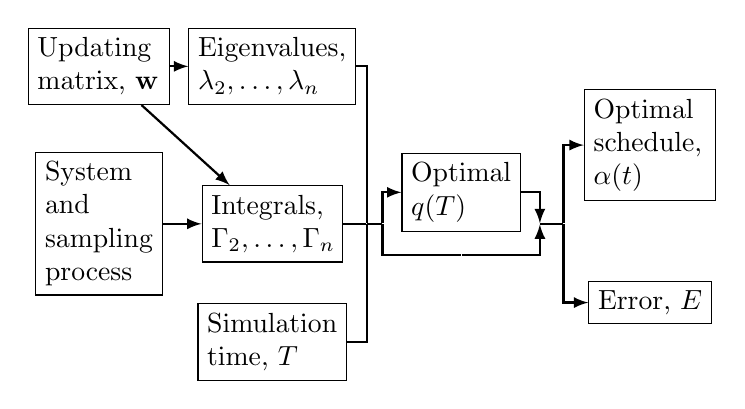
\begin{tikzpicture}
  \node[draw, text width={width("Updating ")}]
    (w) at (0, 3) {Updating \\matrix, $\mathbf w$};

  \node[draw, text width={width("sampling")}]
    (sys) at (0, 1) {System\\and\\sampling\\process};

  \node[draw, text width={width("Eigenvalues,")}]
    (lambda) at (2.2, 3) {Eigenvalues,\\$\lambda_2, \dots, \lambda_n$};

  \node[draw, text width={width("Integrals, ")}]
    (gamma) at (2.2, 1) {Integrals, \\$\Gamma_2, \dots, \Gamma_n$};

  \node[draw, text width={width("Simulation")}]
    (T) at (2.2, -0.5) {Simulation\\time, $T$};

  \node[draw, text width={width("Optimal")}]
    (qT) at (4.6, 1.4) {Optimal\\ $q(T)$};

  \node[draw, text width={width("Schedule,")}]
    (alpha) at (7, 2) {Optimal schedule,\\ $\alpha(t)$};

  \node[draw, text width={width("Error, $\Err$")}]
    (err) at (7, 0) {Error, $\Err$};

  \node[inner sep=0, minimum size=0] (M1) at (3.4, 1) {};

  \node[inner sep=0, minimum size=0] (N1) at (5.9, 1) {};

  \node[inner sep=0, minimum size=0] (R1) at (3.6, 1) {};
  \node[inner sep=0, minimum size=0] (R2) at (4.6, 0.6) {};
  \node[inner sep=0, minimum size=0] (R3) at (5.6, 1) {};

  \draw[->, >=latex, thick]
    (w) edge (lambda)
    (w) edge (gamma)
    (sys) edge (gamma);

  \draw[->, >=latex, thick]
    (lambda) -| (M1)
    (gamma)  -- (M1)
    (T)      -| (M1)
    (M1)     -- (R1)
    (R1)     |- (qT);

  \draw[->, >=latex, thick]
    (qT)     -| (R3);

  \draw[->, >=latex, thick]
    (R3) -- (N1) |- (alpha);

  \draw[->, >=latex, thick]
    (N1) |- (err);

  \draw[->, >=latex, thick]
    %(M1) edge[bend left=70] (N1);
    (R1) |- (R2) -| (R3);
\end{tikzpicture}
\caption{
  \label{fig:vardep}
  Dependence of variables in computing
  the optimal schedule and the error.
}
\end{figure}




\begin{enumerate}

\item
From the updating matrix, $\mathbf w$,
compute the eigenvalues, $\lambda_k$'s.

\item
Run a preliminary adaptive FDS simulation
%using the updating scheme
with a constant updating magnitude, $\alpha_0$.

\item
Compute $\Gamma_k$'s from Eq. \eqref{eq:varY}.

\item
Compute $q(T)$ from the root of Eq. \eqref{eq:opt_qT}.

\item
Compute the optimal schedule by
numerically integrating Eq. \eqref{eq:q_opt}.

\item
Compute the error $E$ from
Eqs. \eqref{eq:error_split},
  \eqref{eq:error_res1},
  and
  \eqref{eq:error_asym2}.

\end{enumerate}







\section{\label{sec:stabilize_wband}
Stabilization of homogeneous updating schemes}



%A practical problem of using homogeneous updating scheme
%is the following.
%
A homogeneous updating scheme
specified by an arbitrary kernel
is not necessarily stable,
i.e., some eigenvalues may be negative.
%
%
%\note{
  %For example,
  %the triple-bin updating scheme
  %is unstable if Eq. \eqref{eq:nn_stable} is violated.
  %
  Even
  the Gaussian updating scheme can be unstable
  in practice
  if the updating kernel is truncated.
%}%
%
Here we show how to minimally modify
the updating kernel
to stabilize it.
%
\note{The relative code is \texttt{trimwindow()} in \texttt{invt.h}.
}


Given an updating kernel,
we can compute the eigenvalues from
Eq. \eqref{eq:wband_eigenvalue}.
%
By replacing negative eigenvalues with zeros and
using Eq. \eqref{eq:mu_from_lambda_pbc}
or \eqref{eq:mu_from_lambda_refl},
we get a new updating kernel,
which is stable by construction.
%
However, the new kernel is widened
as $\mu_l$ may be nonzero for $l > b$.
%
If we truncate the new kernel at $\mu_b$,
the stability problem remains,
although the negative eigenvalues
often become smaller in magnitude.
%
Thus, to stabilize the updating kernel
without increasing the width,
we need to iterate the above process many times,
resulting the following algorithm.


%
\begin{enumerate}
  \item
    Given an updating kernel, $\mu_0, \dots, \mu_b$,
    compute the eigenvalues
    $\lambda_1, \dots, \lambda_n$
    from Eq. \eqref{eq:wband_eigenvalue}.
  \item
    If all eigenvalues are nonnegative,
    we are done, and exit the loop.
  \item
    Otherwise, replace negative eigenvalues by zeros,
    and compute the new kernel,
    $\mu_0, \dots, \mu_b$, from
    Eq. \eqref{eq:mu_from_lambda_pbc}
    or
    \eqref{eq:mu_from_lambda_refl}
    with $\mu_l = 0$ for $l > b$.
    Go to step 1.
\end{enumerate}



\section{\label{sec:equilerr}
Error of the ideal equilibrium FDS simulation}



%As discussed in Sec. \ref{sec:FDS},
%the asymptotic limit of an adaptive FDS method
%is the corresponding equilibrium FDS method
%with the bias potential fixed to the exact value.
%%
%Such a simulation delivers the maximal efficiency.

In late stages of an adaptive FDS simulation,
the bias potential is often sufficiently precise.
Some practitioners would then fix
the bias potential and switch
to the equilibrium method
to prevent possible future efficiency loss
due to the adaptive updates.
%
Below, we shall show that this practice is unnecessary
if the simulation uses the single-bin updating scheme
with the optimal schedule, Eq. \eqref{eq:alpha_invt1}.
%
That is, the bias potential obtained from
an optimal single-bin scheme adaptive simulation
will be similar in precision to that from
the ideal equilibrium simulation
for long times.
%
%Thus, our demonstration below serves as an alternative proof
%of the optimality of the single-bin scheme.

The error of the equilibrium FDS simulation
depends on the precision of the histogram.
%
If all $v_i$'s are exact,
the error is minimized, and can be computed
from the second term
on the right-hand side of Eq. \eqref{eq:vcorr_equil},
%
\begin{align}
  E
  &=
  \left\langle
    \sum_{ i = 1 }^ n
      \rho_i \,
      \left(
        \ln \frac { H_i }
                  { p_i }
        -
        \sum_{r = 1}^n \rho_r
        \ln \frac { H_r }
                  { p_r }
      \right)^2
  \right\rangle
  \notag
  \\
  &
  \approx
  \sum_{ i = 1 }^ n
    \rho_i \,
    \left\langle
      \left(
        \frac { H_i }
              { p_i }
        -
        \sum_{r = 1}^n \rho_r
            \frac { H_r }
                  { p_r }
      \right)^2
    \right\rangle,
\notag
\end{align}
where
$H_i = \frac{1}{T} \sum_{t = 1}^T h_i(t)$
with
$h_i(t)$ defined by Eq. \eqref{eq:h_def}.

We can rewrite the error as
a sum of the eigenmode as
%
\begin{align}
  E
  =
  \sum_{ k = 2 }^n
    \left\langle
      \Theta_k^2
    \right\rangle
  ,
\notag
%\label{eq:error_sbin_equil}
\end{align}
%
where
%
$
  \Theta_k
  =
  \frac{ 1 } { T }
  \sum_{ t = 1 } ^ T
    \theta_k( t )
  ,
$
%
with $\theta_k(t)$ defined by Eq. \eqref{eq:eta_def}.
%and $\phi_{k i}$ by Eq. \eqref{eq:eig_orthonormal_cols}.
%\begin{align}
%\theta_k( t )
%=
%\sum_{ i = 1 }^ n
%\phi_{k i} \left[
%             \frac{ h_i(t) }
%                  { p_i    }
%             - 1
%           \right],
%\end{align}
%and
%\begin{align}
%\sum_{ k = 1 }^n
%  \phi_{k i} \, \phi_{k j}
%  = p_i \, \delta_{i j}.
%\end{align}
%
\note{Because
%
\begin{align*}
  \sum_{ k = 1 }^n
    \Theta_k^2
  &=
  \frac{ 1 } { T^2 }
  \sum_{ t, t' = 1 }^T
    \sum_{ k = 1 }^n
      \theta_k( t ) \, \theta_k( t' )
  \\
  &=
  \frac{ 1 } { T^2 }
  \sum_{ t, t' = 1 }^T
    \sum_{ i, j = 1 }^n
      \xi_i(t) \, \xi_j(t')
      %\left[
      %  \frac{ h_i(t) }
      %       { p_i    }
      %  - 1
      %\right]
      %\left[
      %  \frac{ h_j(t') }
      %       { p_j     }
      %  - 1
      %\right]
      \sum_{ k = 1 }^n
        \phi_{k \, i} \, \phi_{k \, j}
  \\
  &=
  \frac{ 1 } { T^2 }
  \sum_{ t, t' = 1 }^T
    \sum_{ i, j = 1 }^n
      \xi_i(t) \, \xi_j(t') \,
      \rho_i \, \delta_{i, j}
  \\
  &=
  \sum_{ i = 1 }^n
  \frac{ 1 } { T }
  \sum_{ t = 1 }^T \xi_i(t)
  \;
  \frac{ 1 } { T }
  \sum_{ t' = 1 }^T \xi_i(t')
  \\
  &=
  \sum_{ i = 1 }^n
    \rho_i \,
      \left(
        \frac{ H_i }
             { p_i }
        -
        \sum_{r = 1}^n \rho_r
        \frac{ H_r }
             { p_r }
      \right)^2
  ,
\end{align*}
where we have used
$$
  \frac{1}{T}
  \sum_{t = 1}^T \xi_i(t)
  =
  \frac{ H_i }
       { p_i }
  -
  \sum_{r = 1}^n \rho_r
  \frac{ H_r }
       { p_r }
  .
$$
}%
The sum starts from $k = 2$, for
by Eq. \eqref{eq:eigenmode1}, % we have
$$
\theta_1(t)
=
\sum_{ i = 1 }^n
  \phi_{1i} \, \left(
    \frac{ h_i(t) } { p_i }
    -
    \sum_{r = 1}^n
    \rho_r
    \frac{ h_r(t) } { p_r }
  \right)
= 0.
$$

In the long-time limit,
\begin{align*}
  \left\langle
    \Theta_k^2
  \right\rangle
  &=
  \frac{1}{T^2}
  \sum_{ t, t' = 1 }^T
  \langle \theta_k(t) \, \theta_k(t') \rangle
  %\\
  %&\approx
  %\frac{1}{T}
  %\sum_{ \tau = -\infty }^{ \infty }
  %\langle \theta_k(t) \, \theta_k(t + \tau) \rangle
  %\\
  %&=
  =
  \frac{1}{T}
  \sum_{\tau = -\infty}^\infty
    \kappa_n(\tau)
  =
  \frac{ \Gamma_k }{ T }
.
\end{align*}
%
Thus,
\begin{equation}
  E
  =
  \frac{ 1 } { T }
  \sum_{ k = 2 }^n \Gamma_k
  .
\label{eq:error_equil}
\end{equation}

Now comparing this with the error of
the optimal adaptive simulation,
Eq. \eqref{eq:error_sinc} (with $K = n$),
we find the difference to be negligible
in the long time limit.

The above argument can be extended
to the bandpass updating schemes.
%
If the intrinsic PMF is sufficiently smooth,
we can explicitly filter out some error modes
in the histogram,
say those with $k >  K$,
and truncate the sum in
Eq. \eqref{eq:error_equil} at $k = K$.






\section{\label{sec:invt_schedule}
Modified inverse-time schedules}



As an alternative to the
optimal schedule from Eq. \eqref{eq:q_opt},
here we consider the modified
inverse-time formula, Eq. \eqref{eq:alpha_invtlambda},
%with a free parameter $\lambda$.
%
whose error can be computed explicitly.



\subsection{\label{sec:invt_error}
Error
}



Using Eq. \eqref{eq:alpha_invtlambda}
in Eq. \eqref{eq:error_asym1} yields
%
\begin{align}
  \Err_A
  &=
  \frac{    1    }
       { T + t_0 }
  \sum_{k = 2}^n
    \frac{ \Gamma_k \, \nu_k^2 }
         {    2 \, \nu_k - 1   }
  \left[
    1 - \left(
          \frac {     t_0 }
                { T + t_0 }
        \right)^{ 2 \, \nu_k - 1 }
  \right]
  ,
\label{eq:error_asym_invt}
\end{align}
%
where $\nu_k \equiv \lambda_k / \lambda$.
%
From Eq. \eqref{eq:error_res1},
we get
%
\begin{equation}
  \Err_R
  =
  \frac { \alpha_0 } { 2 }
  \sum_{k = 2}^n
  \Gamma_k \, \lambda_k \,
  \left(
      \frac{   t_0   }
           { T + t_0 }
  \right)^{ 2 \, \nu_k }
  .
\notag
%\label{eq:error_res_invt}
\end{equation}
%
The total error is the sum of the two.
%with
%$
%  q(T)
%  =
%  ( 1 / \lambda )
%  \ln\left(
%    1 + T / t_0
%  \right)
%$
%%
%from integrating Eq. \eqref{eq:alpha_invtlambda}.
%
%We assume that
%the system was initially equilibrated
%at a constant $\alpha_0$,
%such that the values of
%$\left\langle y_k^2(0) \right\rangle$
%can be computed from Eq. \eqref{eq:y2_eql},
%as well as Eq. \eqref{eq:t0_sinc}.
%
%The total error is
%%
%\begin{align}
%\Err
%&=
%\Err_R + \Err_A
%\notag
%\\
%&=
%\sum_{ k = 2 }^n
%  \frac
%  {
%    \Gamma_k \, \nu_k \,
%    \left[
%      \nu_k
%      +
%      (\nu_k - 1)
%      \left(
%        \frac{ t_0 } { T + t_0 }
%      \right)^{ 2 \, \nu_k - 1 }
%    \right]
%  }
%  {
%    (T + t_0) \, (2 \, \nu_k - 1)
%  }
%  .
%%\notag
%\label{eq:error_invt}
%\end{align}




\subsection{\label{sec:invt_singlebin}
  Single-bin updating scheme
}



For the single-bin scheme, we have
$\lambda_2 = \cdots = \lambda_n = 1$,
and
$\Gamma_k$'s affect the error
only via the sum, $\sum_{k = 2}^n \Gamma_k$,
as a multiplicative constant.

In the asymptotic limit,
we can focus on the asymptotic error
and drop the second term in the square brackets
of Eq. \eqref{eq:error_asym_invt}
by assuming $\lambda < 2$.
%
Then,
$$
  E_A
  =
  \frac { 1 } { T + t_0 }
  \frac {             1            }
        { \lambda \, (2 - \lambda) }
  \sum_{ k = 2 }^n \Gamma_k
  ,
$$
is minimal at $\lambda = 1$.
%
\note{A higher-order correction:
  $
  \lambda = 1 -
  \left[
    1 - \frac 1 2 \alpha_0 \, (T+t_0)
  \right] r \, \log r
  ,
  $
  where $r = t_0 / (T + t_0)$.
}




\subsection{\label{sec:invt_nn}
Triple-bin updating scheme}




For the triple-bin updating scheme,
%introduced in Sec. \ref{sec:nnscheme},
we can find an analytical expression
of the optimal value of $\lambda$
in the large-$n$ and asymptotic limit.
%
In this case,
if $2 \, \nu_k > 1$ for every $k$,
the asymptotic error is given by the integral
%$\sum_i \to \frac{2 \, n}{\pi} \int_0^{\pi/2} dp$, and
%
\begin{align}
  \Err_A
  =
  \frac{ 2 \, n  }
       { \pi \, T }
  \int_0^{\pi/2}
    \frac{ \Gamma(p) \, \left(1 - 4 \, \mu_1 \, \sin^2 p \right)^2    }
         {   \lambda \, \left(2 - 8 \, \mu_1 \, \sin^2 p - \lambda \right) }
  \, dp
  .
\notag
%\label{eq:error_nn_asym_int}
\end{align}



For perfect sampling,
$\Gamma(p) = 1$ from Eq. \eqref{eq:Gamma_perfect},
and
$$
\begin{aligned}
  \Err_A
  &=
  \frac{n}{4 \, T}
  \left(
    \frac{2 - 4 \, \mu_1 + \lambda}{ \lambda }
    +
    \frac{ \lambda }
    { \sqrt{ (2 - \lambda) (2 - 8 \, \mu_1 - \lambda) } }
  \right)
.
\end{aligned}
$$
%
Minimizing the function yields
%
\begin{equation}
  \lambda
  =
  \frac{ 1 - 4 \, \mu_1 }
       { 1 - 2 \, \mu_1 }
  ,
%\notag
\label{eq:lambda_nn_perfect}
\end{equation}
%
and the asymptotic error in the optimal case is given by
%
\begin{equation}
  \Err_A
  =
  \frac{n}{T}
  \left(
    1+ \frac{2 \, \mu_1^2}{1-4 \, \mu_1}
  \right)
  ,
\notag
%\label{eq:error_nn_perfect}
\end{equation}
%
%From Eq. \eqref{eq:error_nn}, it is clear that
which
is minimal at $\mu_1 = 0$, the single-bin case.
%increases with the magnitude of $\mu_1$
%no matter its sign,
%and the minimal value, obtained at $\mu_1 = 0$,
%corresponds to the single-bin scheme.
%
Note that the value given by
Eq. \eqref{eq:lambda_nn_perfect}
was less than the observed optimal value
from Fig. \ref{fig:errinvt},
and the latter would decrease
with the simulation length.
%




For the one-step sampling process,
we find from Eq. \eqref{eq:Gamma_onestep}
that $\Gamma(p) = \cot^2 p$
peaks around $p \approx 0$,
%
Then
$$
  \Err_A
  \propto
  \frac{   2 \, n }
       { \pi \, T }
  \frac{             1             }
       {  \lambda \, (2 - \lambda) }
  .
$$
%
The optimal $\lambda$ is, therefore,
%
$
%\begin{equation}
  \lambda \approx 1.
%\label{eq:lambda_nn_onestep}
%\end{equation}
$
%

\note{
However, the above result %Eq. \eqref{eq:lambda_nn_onestep}
is only good
for sufficiently short simulations,
since we have taken the limit of $n \to \infty$
for a fixed $T$.
%
For very long simulations,
the optimal $\lambda$
will ultimately drift to
the smallest eigenvalue,
$\min \lambda_k = 1 - 4 \, \mu_1$.
}



\bibliography{simul}
\end{document}
